% =====================================================================
%  TALS Physik - Formelsammlung (RLP-BM 2030)
%  Berufsmaturitaet Technik, Architektur, Life Sciences
%
%  Aufbau folgt den Themenseiten von go4exercises.github.io/TALS-Physik:
%    0  Mathematischer Werkzeugkasten (aus den Vorwissen-Seiten)
%    4  Mechanik        (4.1 - 4.5)
%    5  Thermodynamik   (5.1 - 5.3)
%    6  Wellen und Elektrizitaet (6.1, 6.2)
%    A  Anhang: Konstanten, Stoffwerte, Einheiten
%
%  Lizenz: CC BY-NC 4.0 · Haftungsausschluss am Dokumentende
%  Konventionen: Schweizer Hochdeutsch (kein Eszett), Dezimalpunkt,
%  Skalare kursiv, Vektoren mit Pfeil, Einheiten aufrecht,
%  Bernstein-Farbschema #8A4A0E, alle Skizzen parametrisiert (TikZ).
%
%  Uebersetzen:  pdflatex formelsammlung.tex   (zweimal, wegen Inhaltsverzeichnis)
%  Benoetigt:    tikz, needspace, fancyhdr, xcolor, geometry, multicol,
%                enumitem, hyperref, amsmath
%  Hinweis: babel wird mit [provide=*] geladen, damit die Datei auch ohne
%  installierte ngerman-Trennmuster uebersetzt.
%
%  Satzspiegel je Formel-Eintrag:
%      \ftitel{Titel}                        <- volle Breite
%      \begin{minipage}[t]{0.54\linewidth}   <- LINKS: Formel(n), linksbuendig
%          \[ ... \]  \hinweis{...}            (fleqn, \mathindent = 0pt)
%      \end{minipage}\hfill
%      \begin{minipage}[t]{0.44\linewidth}   <- RECHTS: Legende + Skizze
%          \begin{leg} ... \end{leg}
%          {\centering\tikzfont <tikzpicture> \fcap{...}\par}
%      \end{minipage}
%
%  Struktur-Makros:  \LG{Nr}{Lerngebiet}   \TG{Nr}{Teilgebiet}
%                    \ftitel{Formeltitel}  leg-Umgebung (Legende)
%                    \hinweis{...}  \fcap{Skizzen-Bildunterschrift}
% =====================================================================
\documentclass[10pt,a4paper]{article}
\usepackage[T1]{fontenc}
\usepackage{charter}
\usepackage[utf8]{inputenc}
\usepackage[provide=*,ngerman]{babel}
\usepackage[fleqn]{amsmath}
\usepackage{amssymb}
\usepackage{tikz}
\usepackage[table]{xcolor}
\usepackage{geometry}
\usepackage{array}
\usepackage{multicol}
\usepackage{enumitem}
\usepackage{fancyhdr}
\usepackage{needspace}

\usepackage{qrcode}
\newcommand{\talsweb}{https://go4exercises.github.io/TALS-Physik}
\usepackage[hidelinks]{hyperref}
\hypersetup{
  pdftitle={TALS Physik -- Formelsammlung},
  pdfauthor={Raphael Arnold Kohler},
  pdfsubject={Berufsmaturität TALS, RLP-BM 2030},
  pdfkeywords={Physik, Formelsammlung, Berufsmaturität, TALS, RLP-BM 2030},
  pdflang={de-CH}}
\urlstyle{same}
\usetikzlibrary{arrows.meta,decorations.pathmorphing,patterns,calc,angles,quotes}

\setlength{\headheight}{13pt}
\geometry{a4paper,left=14mm,right=14mm,top=15mm,bottom=12mm,headsep=3.5mm,footskip=7mm}

\definecolor{bern}{HTML}{8A4A0E}
\definecolor{bernm}{HTML}{9A5F12}
\definecolor{bernl}{HTML}{F7EFE6}
\definecolor{grau}{HTML}{4A4A4A}
\definecolor{hgrau}{HTML}{6B6B6B}

\pagestyle{fancy}\fancyhf{}
\renewcommand{\headrulewidth}{0.4pt}
\renewcommand{\headrule}{\hbox to\headwidth{\color{bernm}\leaders\hrule height \headrulewidth\hfill}}
\fancyhead[L]{\footnotesize\color{bern}\href{\talsweb/}{\textbf{TALS Physik}} · Formelsammlung \color{hgrau}v1.0}
\makeatletter
\newcounter{talsLG}
\newcommand{\talsfresh}[1]{\expandafter\gdef\csname talsfresh@#1\endcsname{}}
\newcommand{\talsmarkfresh}{\immediate\write\@auxout{\string\talsfresh{\thepage}}}
\newcommand{\tals@L}[2]{#1}
\newcommand{\tals@R}[2]{#2}
\newcommand{\talskopf}{%
  \protected@edef\tals@tm{\topmark}%
  \@ifundefined{talsfresh@\the\c@page}{}{\tals@freshtrue}%
  \iftals@fresh
    \leftmark
  \else
  \ifx\tals@tm\@empty
    \leftmark
  \else
    \protected@edef\tals@a{\expandafter\tals@L\topmark}%
    \protected@edef\tals@b{\leftmark}%
    \ifx\tals@a\@empty
      \leftmark
    \else
      \ifx\tals@a\tals@b
        \leftmark
      \else
        \tals@a\ \textbar\ \tals@b
      \fi
    \fi
  \fi
  \fi
  \tals@freshfalse}
\newif\iftals@fresh
\makeatother
\fancyhead[R]{\footnotesize\color{grau}\talskopf}
\fancyfoot[C]{\footnotesize\color{grau}\thepage}

% Seite 1 hat keine Marke vom Seitenanfang -- dort direkt \leftmark verwenden.
\fancypagestyle{talstitel}{%
  \fancyhf{}%
  \fancyhead[L]{\footnotesize\color{bern}\href{\talsweb/}{\textbf{TALS Physik}} · Formelsammlung \color{hgrau}v1.0}%
  \fancyhead[R]{\footnotesize\color{grau}\leftmark}%
  \fancyfoot[C]{\footnotesize\color{grau}\thepage}}

\setlength{\mathindent}{0pt}
\setlength{\abovedisplayskip}{3pt}
\setlength{\belowdisplayskip}{3pt}
\setlength{\abovedisplayshortskip}{2pt}
\setlength{\belowdisplayshortskip}{2pt}
\setlength{\parindent}{0pt}
\setlength{\parskip}{0pt}

% ---------- Struktur-Makros ----------
\newcommand{\LG}[2]{%
  \par\vspace{1.6mm}\needspace{7\baselineskip}%
  \ifdim\pagetotal=0pt\relax\talsmarkfresh\fi%
  \phantomsection%
  \addcontentsline{toc}{section}{\textbf{#1}\quad #2}%
  \markboth{#1\ \ #2}{}%
  \noindent\colorbox{bern}{\parbox{\dimexpr\linewidth-2\fboxsep\relax}{\vspace{0.4mm}\color{white}\bfseries\large #1\quad #2\vspace{0.4mm}}}%
  \par\vspace{1.6mm}}

\makeatletter
\newcommand{\TG}[3][]{%
  \par\vspace{2.4mm}\needspace{5\baselineskip}\phantomsection%
  \addcontentsline{toc}{subsection}{#2\quad #3}%
  \noindent{\color{bern}\bfseries\normalsize
    \if\relax\detokenize{#1}\relax #2\quad #3\else\href{#1}{#2\quad #3}\fi}%
  \par\vspace{-1.4mm}{\color{bernm}\rule{\linewidth}{0.8pt}}\par\vspace{1.2mm}}
\makeatother

\newcommand{\ftitel}[1]{\par\noindent{\bfseries\footnotesize\color{grau}#1}\par\vspace{0.2mm}\nopagebreak}
\newcommand{\ftitelD}[1]{\par\noindent{\bfseries\footnotesize\color{grau}#1}\par\nopagebreak\vspace{\dimexpr-0.5mm-\baselineskip\relax}\nopagebreak}

\newenvironment{leg}%
  {\par\begingroup\footnotesize\setlength{\tabcolsep}{2.5pt}%
   \renewcommand{\arraystretch}{1.0}%
   \begin{tabular}[t]{@{}>{$}l<{$}@{\ \,}l@{\quad}l@{}}}%
  {\end{tabular}\endgroup\par\vspace{0.3mm}}

\newcommand{\warnsym}{\tikz[baseline=-0.5ex]{\draw[bern,line width=0.45pt] (0,0)--(0.21,0.36)--(0.42,0)--cycle;
  \node at (0.21,0.12) {\tiny\bfseries !};}}
\newcommand{\gilt}[1]{\par\vspace{0.3mm}{\footnotesize\color{grau}\textbf{Gültig:} #1}\par\vspace{0.5mm}}
\newcommand{\warn}[1]{\par\vspace{0.4mm}{\footnotesize\color{bern}\warnsym\ #1}\par\vspace{0.6mm}}
\newcommand{\merk}[1]{\par\vspace{0.7mm}\noindent\colorbox{bernl}{\parbox{\dimexpr\linewidth-2\fboxsep\relax}%
  {\vspace{0.5mm}\footnotesize\color{grau}#1\vspace{0.5mm}}}\par\vspace{0.9mm}}
\newcommand{\hinweis}[1]{\par\vspace{0.4mm}{\footnotesize\color{hgrau}#1}\par\vspace{1.6mm}}

\newcommand{\fcap}[1]{\par\vspace{-1mm}{\scriptsize\color{hgrau}#1}\par}

\newcommand{\ME}[1]{\ensuremath{\mathrm{#1}}}
\newcommand{\anm}[1]{\;\text{\normalfont\footnotesize\color{grau}#1}}
\newcommand{\mtxt}[1]{\text{\small #1}}
% Zwischenüberschrift, der direkt eine Displayformel folgt (unterdrückt die Phantomzeile)
\newcommand{\zwiD}[1]{\par\vspace{0.7mm}\noindent{\footnotesize\color{grau}#1}\par\nopagebreak%
  \vspace{\dimexpr-0.5mm-\baselineskip\relax}\nopagebreak}
% Fliesstext, dem direkt eine Displayformel folgt
\newcommand{\hinweisD}[1]{\par\vspace{0.3mm}{\footnotesize\color{hgrau}#1}\par\nopagebreak%
  \vspace{\dimexpr-0.5mm-\baselineskip\relax}\nopagebreak}
\newcommand{\warnD}[1]{\par\vspace{0.4mm}{\footnotesize\color{bern}\warnsym\ #1}\par\nopagebreak%
  \vspace{\dimexpr-0.5mm-\baselineskip\relax}\nopagebreak}

% ---------- TikZ-Stile ----------
\tikzset{
  vec/.style={-{Latex[length=1.9mm,width=1.4mm]},bern,line width=0.7pt},
  vecg/.style={-{Latex[length=1.9mm,width=1.4mm]},bernm,line width=0.7pt},
  ax/.style={-{Latex[length=1.6mm,width=1.2mm]},grau,line width=0.5pt},
  kurve/.style={bern,line width=0.9pt},
  hilf/.style={hgrau,dashed,line width=0.4pt},
  koerper/.style={fill=bernl,draw=bern,line width=0.6pt},
}
\newcommand{\tikzfont}{\footnotesize}

\begin{document}
\thispagestyle{talstitel}

\begin{center}
  {\color{bern}\LARGE\bfseries Formelsammlung Physik}\\[1.2mm]
  {\color{grau}\normalsize Berufsmaturität Technik, Architektur, Life Sciences\ \ ·\ \ RLP-BM 2030}\\[0.8mm]
  {\color{hgrau}\footnotesize TALS Physik\ \ ·\ \ Lerngebiete 4 Mechanik, 5 Thermodynamik, 6 Wellen \& Elektrizität\ \ ·\ \ mit mathematischem Werkzeugkasten}
\end{center}
\vspace{1mm}
{\color{bernm}\rule{\linewidth}{1pt}}
\vspace{1.5mm}

{\footnotesize
\textbf{Zur Benutzung.} Jede Formel steht mit \textbf{Legende} (Formelzeichen -- Bedeutung -- SI-Einheit). Skizzen und Diagramme sind
\emph{parametrisiert}: sie zeigen die Grössen der Formel, keine Zahlenbeispiele. Schreibweisen: Dezimal\textbf{punkt} (\(9.81\;\ME{m/s^2}\)),
Skalare kursiv (\(v,\,a,\,F\)), Vektoren mit Pfeil (\(\vec F\)), Einheiten aufrecht.
\textbf{Für Prüfungen gelten die von Schule, Kanton oder Prüfungsleitung festgelegten Hilfsmittel} -- vor jeder Prüfung prüfen,
welche Formelsammlung zugelassen ist.
\par}
\vspace{2mm}

\begingroup
\renewcommand{\contentsname}{\vspace{-6mm}}
\setlength{\columnsep}{8mm}
{\footnotesize
\begin{multicols}{3}
\tableofcontents
\end{multicols}}
\endgroup

% ======================================================================
\LG{0}{Mathematischer Werkzeugkasten}\TG[https://go4exercises.github.io/TALS-Physik/themen/p0-1-vorwissen-mathematik.html\#proportional]{0.1}{Proportionalität}\begin{minipage}[t]{0.54\linewidth}\vspace{0pt}
\ftitelD{Direkte Proportionalität}
\[ y = k\cdot x \qquad\Longleftrightarrow\qquad \frac{y}{x}=k=\mtxt{konst.} \]
\hinweis{Doppeltes \(x\) \(\to\) doppeltes \(y\). Graph: Gerade durch den Ursprung mit Steigung \(k\). Kurzschreibweise \(y\sim x\).}
\end{minipage}\hfill
\begin{minipage}[t]{0.44\linewidth}\vspace{0pt}
\begin{leg}
x,y & zwei Grössen & je nach Grösse\\
k & Proportionalitätsfaktor & \([y]/[x]\)
\end{leg}
{\centering\tikzfont
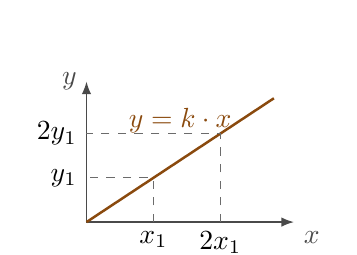
\begin{tikzpicture}[scale=0.85]
  \draw[ax] (0,0)--(3.1,0) node[below right]{$x$};
  \draw[ax] (0,0)--(0,2.1) node[left]{$y$};
  \draw[kurve] (0,0)--(2.8,1.85);
  \node[bern] at (1.4,1.52) {$y=k\cdot x$};
  \draw[hilf] (1.0,0)--(1.0,0.66)--(0,0.66);
  \draw[hilf] (2.0,0)--(2.0,1.32)--(0,1.32);
  \node[below] at (1.0,0) {$x_1$}; \node[below] at (2.0,0) {$2x_1$};
  \node[left] at (0,0.66) {$y_1$}; \node[left] at (0,1.32) {$2y_1$};
\end{tikzpicture}
\fcap{direkt: Gerade durch den Ursprung}
\par}
\end{minipage}
\par\vspace{1.6mm}

\begin{minipage}[t]{0.54\linewidth}\vspace{0pt}
\ftitelD{Indirekte (umgekehrte) Proportionalität}
\[ y = \frac{k}{x} \qquad\Longleftrightarrow\qquad x\cdot y = k = \mtxt{konst.} \]
\hinweis{Doppeltes \(x\) \(\to\) halbes \(y\). Graph: Hyperbel. Prüffrage: ist der \emph{Quotient} konstant (direkt) oder das \emph{Produkt} (indirekt)?}
\end{minipage}\hfill
\begin{minipage}[t]{0.44\linewidth}\vspace{0pt}
{\centering\tikzfont
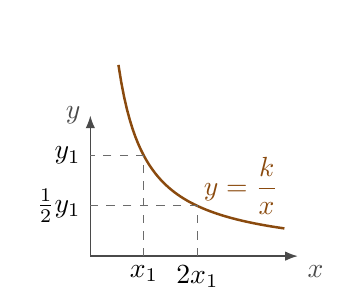
\begin{tikzpicture}[scale=0.85]
  \draw[ax] (0,0)--(3.1,0) node[below right]{$x$};
  \draw[ax] (0,0)--(0,2.1) node[left]{$y$};
  \draw[kurve,domain=0.42:2.9,samples=60,variable=\x] plot ({\x},{1.2/\x});
  \node[bern] at (2.25,1.05) {$y=\dfrac{k}{x}$};
  \draw[hilf] (0.8,0)--(0.8,1.5)--(0,1.5);
  \draw[hilf] (1.6,0)--(1.6,0.75)--(0,0.75);
  \node[below] at (0.8,0) {$x_1$}; \node[below] at (1.6,0) {$2x_1$};
  \node[left] at (0,1.5) {$y_1$}; \node[left] at (0,0.75) {$\tfrac{1}{2}y_1$};
\end{tikzpicture}
\fcap{indirekt: Hyperbel, \(x\cdot y\) konstant}
\par}
\end{minipage}
\par\vspace{1.6mm}

\needspace{4\baselineskip}\ftitelD{Dreisatz}
\[ \frac{y_1}{x_1}=\frac{y_2}{x_2}\quad\Rightarrow\quad y_2 = y_1\cdot\frac{x_2}{x_1} \]
\hinweis{Nur bei direkter Proportionalität. Bei indirekter: \(y_2 = y_1\cdot\dfrac{x_1}{x_2}\).}

\TG[https://go4exercises.github.io/TALS-Physik/themen/p0-1-vorwissen-mathematik.html\#geometrie]{0.2}{Flächen und Volumen}\begin{minipage}[t]{0.54\linewidth}\vspace{0pt}
\ftitelD{Flächen}
\[ A_{\text{Rechteck}} = a\cdot b \qquad A_{\text{Dreieck}} = \tfrac{1}{2}\,g\cdot h_g \qquad A_{\text{Kreis}} = \pi\cdot r^{\,2} \]
\end{minipage}\hfill
\begin{minipage}[t]{0.44\linewidth}\vspace{0pt}
\begin{leg}
A & Fläche & m\(^2\)\\
a,b & Seitenlängen & m\\
g,h_g & Grundseite und zugehörige Höhe & m\\
r & Radius, \(r=d/2\) & m
\end{leg}
{\centering\tikzfont
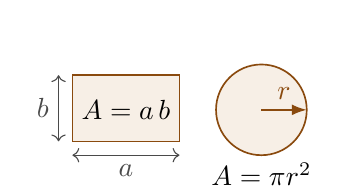
\begin{tikzpicture}[scale=0.8]
  \draw[koerper] (0,0) rectangle (1.7,1.05);
  \draw[<->,grau,line width=0.4pt] (0,-0.22)--(1.7,-0.22) node[midway,below]{$a$};
  \draw[<->,grau,line width=0.4pt] (-0.22,0)--(-0.22,1.05) node[midway,left]{$b$};
  \node at (0.85,0.5) {$A=a\,b$};
  \begin{scope}[xshift=3.0cm,yshift=0.5cm]
    \draw[koerper] (0,0) circle (0.72);
    \draw[vec] (0,0)--(0.72,0) node[midway,above]{$r$};
    \node at (0,-1.02) {$A=\pi r^2$};
  \end{scope}
\end{tikzpicture}
\par}
\end{minipage}
\par\vspace{1.6mm}

\begin{minipage}[t]{0.54\linewidth}\vspace{0pt}
\ftitelD{Volumen}
\[ V_{\text{Quader}} = a\cdot b\cdot c \qquad V_{\text{Zylinder}} = \pi\cdot r^{\,2}\cdot h = A_{\text{Grund}}\cdot h \]
\end{minipage}\hfill
\begin{minipage}[t]{0.44\linewidth}\vspace{0pt}
\begin{leg}
V & Volumen & m\(^3\)\\
h & Höhe & m\\
A_{\text{Grund}} & Grundfläche & m\(^2\)
\end{leg}
{\centering\tikzfont
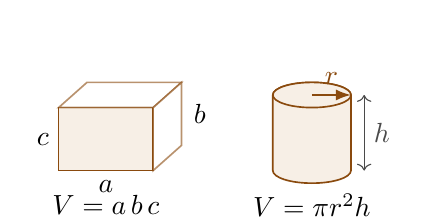
\begin{tikzpicture}[scale=0.8]
  \draw[koerper] (0,0)--(1.5,0)--(1.5,1.0)--(0,1.0)--cycle;
  \draw[koerper,fill=white,opacity=0.6] (0,1.0)--(0.45,1.4)--(1.95,1.4)--(1.5,1.0)--cycle;
  \draw[koerper,fill=white,opacity=0.6] (1.5,0)--(1.95,0.4)--(1.95,1.4)--(1.5,1.0)--cycle;
  \node[below] at (0.75,0) {$a$}; \node[left] at (0,0.5) {$c$};
  \node[right] at (1.99,0.9) {$b$};
  \node at (0.75,-0.55) {$V=a\,b\,c$};
  \begin{scope}[xshift=3.4cm]
    \draw[koerper] (0,0) arc (180:360:0.62 and 0.2) -- (1.24,1.2) arc (0:180:0.62 and 0.2) -- cycle;
    \draw[koerper] (0.62,1.2) ellipse (0.62 and 0.2);
    \draw[vec] (0.62,1.2)--(1.24,1.2) node[midway,above]{$r$};
    \draw[<->,grau,line width=0.4pt] (1.45,0)--(1.45,1.2) node[midway,right]{$h$};
    \node at (0.62,-0.55) {$V=\pi r^2 h$};
  \end{scope}
\end{tikzpicture}
\par}
\end{minipage}
\par\vspace{1.6mm}

\needspace{4\baselineskip}\begin{minipage}[t]{0.54\linewidth}\vspace{0pt}
\ftitelD{Volumeneinheiten}
\[ 1\;\ME{m^3} = 1000\;\ME{l}\qquad 1\;\ME{dm^3}=1\;\ME{l}\qquad 1\;\ME{cm^3}=1\;\ME{ml} \]
\hinweis{Ein Würfel mit \(1\;\ME{dm}\) Kantenlänge fasst genau einen Liter -- daraus folgen alle anderen Litermasse.}
\end{minipage}\hfill
\begin{minipage}[t]{0.44\linewidth}\vspace{0pt}
{\centering\tikzfont
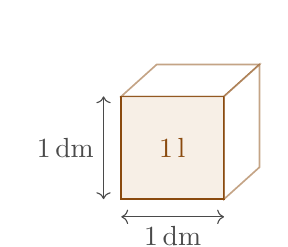
\begin{tikzpicture}[scale=0.9]
  \draw[koerper] (0,0)--(1.45,0)--(1.45,1.45)--(0,1.45)--cycle;
  \draw[koerper,fill=white,opacity=0.5] (0,1.45)--(0.5,1.9)--(1.95,1.9)--(1.45,1.45)--cycle;
  \draw[koerper,fill=white,opacity=0.5] (1.45,0)--(1.95,0.45)--(1.95,1.9)--(1.45,1.45)--cycle;
  \draw[<->,grau,line width=0.4pt] (-0.25,0)--(-0.25,1.45) node[midway,left]{$1\,\ME{dm}$};
  \draw[<->,grau,line width=0.4pt] (0,-0.25)--(1.45,-0.25) node[midway,below]{$1\,\ME{dm}$};
  \node[bern] at (0.72,0.72) {$1\,\ME{l}$};
\end{tikzpicture}
\fcap{Würfel mit 1 dm Kante \(=\) 1 Liter}
\par}
\end{minipage}
\par\vspace{1.6mm}

\begin{minipage}[t]{0.34\linewidth}\vspace{0pt}
\ftitel{Einheitentreppe}
\hinweis{Eine Stufe bedeutet bei \emph{Längen} den Faktor 10, bei \emph{Flächen} 100 und bei \emph{Volumen} 1000 --
die Umrechnungszahl wird mitquadriert bzw.\ hoch drei genommen.}
\merk{Häufigster Fehler: mit 10 statt mit 100 oder 1000 umrechnen.}
\end{minipage}\hfill
\begin{minipage}[t]{0.64\linewidth}\vspace{0pt}
{\centering\tikzfont
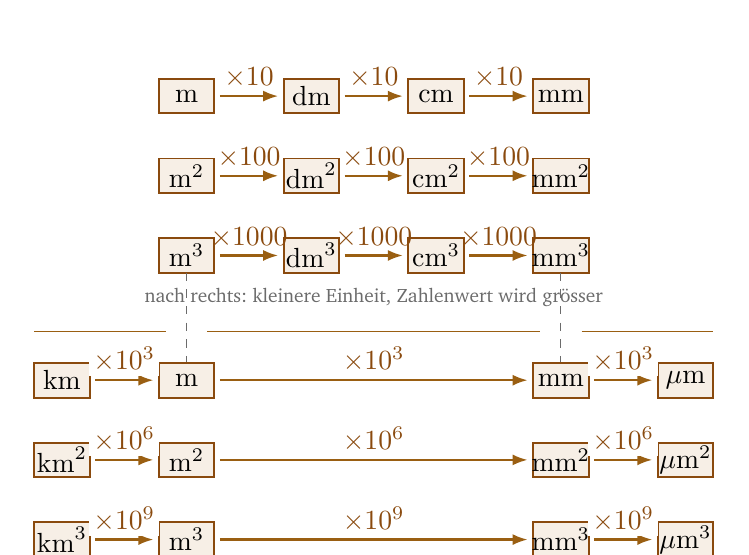
\begin{tikzpicture}[scale=0.88]
  % ===== obere Treppe: m -- dm -- cm -- mm (unveraendert) =====
  \foreach \z/\hoch/\fak in {0/{}/{\times 10}, 1/{^2}/{\times 100}, 2/{^3}/{\times 1000}}{
    \begin{scope}[yshift=-\z*1.15cm]
      \foreach \k/\e in {0/{m}, 1/{dm}, 2/{cm}, 3/{mm}}{
        \draw[koerper,line width=0.7pt] (\k*1.80,0) rectangle (\k*1.80+0.80,0.50);
        \node at (\k*1.80+0.40,0.25) {$\mathrm{\e}\hoch$};}
      \foreach \k in {0,1,2}{
        \draw[vecg,line width=0.8pt] (\k*1.80+0.88,0.25)--(\k*1.80+1.72,0.25);
        \node[bern,above,inner sep=1.5pt] at (\k*1.80+1.30,0.30) {$\fak$};}
    \end{scope}}
  \node[hgrau,font=\scriptsize] at (3.10,-2.66) {nach rechts: kleinere Einheit, Zahlenwert wird grösser};
  % ===== Trennlinie mit Lücken für die Fluchtlinien =====
  \draw[bernm,line width=0.4pt] (-1.80,-3.15)--(0.10,-3.15);
  \draw[bernm,line width=0.4pt] (0.70,-3.15)--(5.50,-3.15);
  \draw[bernm,line width=0.4pt] (6.10,-3.15)--(8.00,-3.15);
  % ===== Fluchtlinien: m und mm stehen übereinander =====
  \draw[hgrau,dashed,line width=0.4pt] (0.40,-2.30)--(0.40,-3.60);
  \draw[hgrau,dashed,line width=0.4pt] (5.80,-2.30)--(5.80,-3.60);
  % ===== untere Treppe: km -- m -- mm -- µm, Mitte auseinandergezogen =====
  \foreach \z/\hoch/\fak in {0/{}/{\times 10^{3}}, 1/{^2}/{\times 10^{6}}, 2/{^3}/{\times 10^{9}}}{
    \begin{scope}[yshift=-4.10cm-\z*1.15cm]
      \foreach \x/\e in {-1.80/{km}, 0.00/{m}, 5.40/{mm}, 7.20/{\mu m}}{
        \draw[koerper,line width=0.7pt] (\x,0) rectangle (\x+0.80,0.50);
        \node at (\x+0.40,0.25) {$\mathrm{\e}\hoch$};}
      \foreach \x/\y in {-1.00/0.00, 0.80/5.40, 6.20/7.20}{
        \draw[vecg,line width=0.8pt] (\x+0.08,0.25)--(\y-0.08,0.25);
        \node[bern,above,inner sep=1.5pt,fill=white] at ({(\x+\y)/2},0.30) {$\fak$};}
    \end{scope}}
\end{tikzpicture}
\fcap{Vorsatz-Treppe in Tausenderschritten -- die obere Treppe löst das Stück von m bis mm im Detail auf}
\par}
\end{minipage}
\par\vspace{1.6mm}

\TG[https://go4exercises.github.io/TALS-Physik/themen/p0-1-vorwissen-mathematik.html]{0.3}{Kreis, Winkel und Bogenmass}\begin{minipage}[t]{0.54\linewidth}\vspace{0pt}
\ftitelD{Umfang}
\[ \pi = \frac{U}{d}\qquad\Longrightarrow\qquad U = \pi\cdot d = 2\pi\cdot r \]
\end{minipage}\hfill
\begin{minipage}[t]{0.44\linewidth}\vspace{0pt}
\begin{leg}
U & Umfang & m\\
d & Durchmesser & m\\
\pi & Kreiszahl \(\approx 3.14159\) & --
\end{leg}
\end{minipage}
\par\vspace{1.6mm}

\begin{minipage}[t]{0.54\linewidth}\vspace{0pt}
\ftitelD{Bogenmass und Grad-Umrechnung}
\[ \varphi_{\text{rad}} = \frac{s_{\mathrm{b}}}{r}\qquad\Longrightarrow\qquad s_{\mathrm{b}} = r\cdot\varphi_{\text{rad}} \]
\[ \varphi_{\text{rad}} = \varphi_{\text{Grad}}\cdot\frac{\pi}{180^\circ}\qquad
   \varphi_{\text{Grad}} = \varphi_{\text{rad}}\cdot\frac{180^\circ}{\pi} \]
\hinweis{Voller Kreis: \(360^\circ \,\widehat{=}\, 2\pi\;\ME{rad}\). Rad ist eine reine Verhältniszahl (m/m).}
\end{minipage}\hfill
\begin{minipage}[t]{0.44\linewidth}\vspace{0pt}
\begin{leg}
\varphi_{\text{rad}} & Winkel im Bogenmass & rad\\
s_{\mathrm{b}} & Bogenlänge & m\\
r & Radius & m
\end{leg}
{\centering\tikzfont
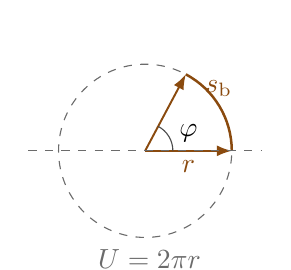
\begin{tikzpicture}[scale=1.1]
  \draw[hilf] (0,0) circle (1.0);
  \draw[kurve] (1,0) arc (0:62:1);
  \draw[vec] (0,0)--(1,0) node[midway,below]{$r$};
  \draw[vec] (0,0)--(62:1);
  \node[bern] at (0.85,0.72) {$s_{\mathrm{b}}$};
  \draw[grau,line width=0.4pt] (0.32,0) arc (0:62:0.32);
  \node at (0.5,0.2) {$\varphi$};
  \draw[hilf] (-1.35,0)--(1.35,0);
  \node[hgrau] at (0.05,-1.25) {$U=2\pi r$};
\end{tikzpicture}
\fcap{\(\varphi\) in rad: Bogen pro Radius}
\par}
\end{minipage}
\par\vspace{1.6mm}

\TG[https://go4exercises.github.io/TALS-Mathe/grundlagen/g5-3-trigonometrische-berechnungen.html]{0.4}{Trigonometrie am Dreieck}\begin{minipage}[t]{0.54\linewidth}\vspace{0pt}
\ftitelD{Winkelfunktionen am rechtwinkligen Dreieck}
\[ \sin\alpha = \frac{a}{c} = \frac{\mtxt{Gegenkathete}}{\mtxt{Hypotenuse}}
   \qquad \alpha = \arcsin\frac{a}{c} \]
\[ \cos\alpha = \frac{b}{c} = \frac{\mtxt{Ankathete}}{\mtxt{Hypotenuse}}
   \qquad \alpha = \arccos\frac{b}{c} \]
\[ \tan\alpha = \frac{a}{b} = \frac{\mtxt{Gegenkathete}}{\mtxt{Ankathete}} = \frac{\sin\alpha}{\cos\alpha}
   \qquad \alpha = \arctan\frac{a}{b} \]
\hinweis{In der Physik überall dort, wo eine Grösse \emph{zerlegt} wird: schiefe Ebene, Kraftkomponenten, Wurf.}
\warn{Taschenrechner auf \textbf{DEG}, wenn der Winkel in Grad gegeben ist -- auf \textbf{RAD},
wenn er im Bogenmass gegeben ist. Ein falscher Modus ist die häufigste Fehlerquelle.}
\end{minipage}\hfill
\begin{minipage}[t]{0.44\linewidth}\vspace{0pt}
\begin{leg}
a & Gegenkathete zu \(\alpha\) & m\\
b & Ankathete zu \(\alpha\) & m\\
c & Hypotenuse & m\\
\alpha & Winkel & \(^\circ\) oder rad
\end{leg}
{\centering\tikzfont
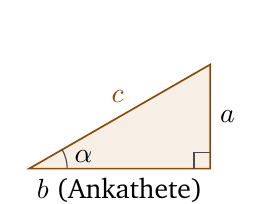
\begin{tikzpicture}[scale=1.15]
  \draw[koerper] (0,0)--(2.0,0)--(2.0,1.15)--cycle;
  \node[below] at (1.0,0) {$b$ (Ankathete)};
  \node[right] at (2.0,0.575) {$a$};
  \node[above left,bern] at (1.15,0.62) {$c$};
  \draw[grau,line width=0.4pt] (0.42,0) arc (0:29.9:0.42);
  \node at (0.6,0.13) {$\alpha$};
  \draw[grau,line width=0.4pt] (1.82,0)--(1.82,0.18)--(2.0,0.18);
\end{tikzpicture}
\fcap{Gegenkathete \(a\) liegt \(\alpha\) gegenüber}
\par}
\end{minipage}
\par\vspace{1.6mm}

\begin{minipage}[t]{0.54\linewidth}\vspace{0pt}
\ftitelD{Schiefwinkliges Dreieck -- Sinus- und Kosinussatz}
\[ \frac{a}{\sin\alpha}=\frac{b}{\sin\beta}=\frac{c}{\sin\gamma}
   \qquad \alpha+\beta+\gamma=180^\circ \]
\[ c^{\,2} = a^{2}+b^{2}-2\,a\,b\,\cos\gamma \]
\hinweisD{Gilt in \emph{jedem} Dreieck. Der Kosinussatz ist der verallgemeinerte Satz des Pythagoras:}
\[ \gamma = 90^\circ:\quad a^2+b^2 = c^2 \quad\Longrightarrow\quad c=\sqrt{a^2+b^2} \]
\hinweis{Denn \(\cos 90^\circ = 0\) -- der letzte Term fällt weg.}
\end{minipage}\hfill
\begin{minipage}[t]{0.44\linewidth}\vspace{0pt}
\begin{leg}
a,b,c & Seiten & m\\
\alpha,\beta,\gamma & Winkel gegenüber \(a,b,c\) & \(^\circ\)
\end{leg}
{\centering\tikzfont
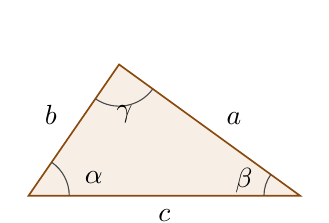
\begin{tikzpicture}[scale=1.15]
  \draw[koerper] (0,0)--(3.0,0)--(1.0,1.45)--cycle;
  \node[below] at (1.5,-0.04) {$c$};
  \node[above left] at (0.42,0.68) {$b$};
  \node[above right] at (2.08,0.68) {$a$};
  \draw[grau,line width=0.4pt] (0.45,0) arc (0:55.4:0.45);
  \node at (0.72,0.20) {$\alpha$};
  \draw[grau,line width=0.4pt] (2.60,0) arc (180:144:0.40);
  \node at (2.38,0.17) {$\beta$};
  \draw[grau,line width=0.4pt] ($(1.0,1.45)+(235.4:0.46)$) arc (235.4:324:0.46);
  \node at (1.06,0.90) {$\gamma$};
\end{tikzpicture}
\fcap{Jeder Seite liegt ihr Gegenwinkel gegenüber: \(a\!\leftrightarrow\!\alpha\), \(b\!\leftrightarrow\!\beta\), \(c\!\leftrightarrow\!\gamma\)}
\par}
\end{minipage}
\par\vspace{1.6mm}

\TG[https://go4exercises.github.io/TALS-Mathe/schwerpunkt/s4-3a-vektorbegriff-komponenten.html]{0.5}{Vektoren}\begin{minipage}[t]{0.54\linewidth}\vspace{0pt}
\ftitelD{Komponenten und Betrag}
\[ F_x = F\cdot\cos\varphi \qquad F_y = F\cdot\sin\varphi \]
\[ F = |\vec F| = \sqrt{F_x^{\,2}+F_y^{\,2}} \qquad \tan\varphi = \frac{F_y}{F_x} \]
\end{minipage}\hfill
\begin{minipage}[t]{0.44\linewidth}\vspace{0pt}
\begin{leg}
\vec F & Vektor (Kraft, Geschw., \dots) & N bzw. m/s\\
F_x,F_y & Komponenten in \(x\)- und \(y\)-Richtung & wie \(\vec F\)\\
\varphi & Winkel zur \(x\)-Achse & \(^\circ\)
\end{leg}
{\centering\tikzfont
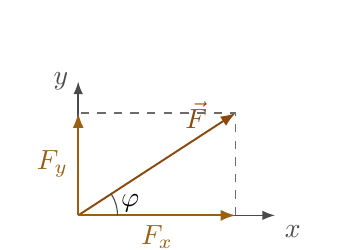
\begin{tikzpicture}[scale=1.0]
  \draw[ax] (0,0)--(2.5,0) node[below right]{$x$};
  \draw[ax] (0,0)--(0,1.7) node[left]{$y$};
  \draw[vec] (0,0)--(2.0,1.3) node[above,pos=0.75]{$\vec F$};
  \draw[hilf] (2.0,0)--(2.0,1.3)--(0,1.3);
  \draw[vecg] (0,0)--(2.0,0) node[midway,below]{$F_x$};
  \draw[vecg] (0,0)--(0,1.3) node[midway,left]{$F_y$};
  \draw[grau,line width=0.4pt] (0.5,0) arc (0:33:0.5);
  \node at (0.66,0.15) {$\varphi$};
\end{tikzpicture}
\par}
\end{minipage}
\par\vspace{1.6mm}

\begin{minipage}[t]{0.54\linewidth}\vspace{0pt}
\ftitelD{Addition (Parallelogramm)}
\[ \vec F_{\mathrm{R}} = \vec F_1 + \vec F_2 \qquad
   F_{R,x}=F_{1,x}+F_{2,x},\quad F_{R,y}=F_{1,y}+F_{2,y} \]
\zwiD{\textbf{Weg 1 -- über die Komponenten.} Die \(x\)-Achse \emph{entlang} \(\vec F_1\) legen; \(\delta\) ist der
Winkel zwischen \(\vec F_1\) und \(\vec F_2\), \(\varphi\) derjenige zwischen \(\vec F_1\) und \(\vec F_{\mathrm{R}}\):}
\[ F_{R,x}=F_1+F_2\cos\delta \qquad F_{R,y}=F_2\sin\delta \qquad
   F_{\mathrm{R}} = \sqrt{F_{R,x}^{\,2}+F_{R,y}^{\,2}} \]
\[ \varphi = \arccos\frac{F_1+F_2\cos\delta}{F_{\mathrm{R}}} \anm{eindeutig für \(0^\circ\le\varphi\le 180^\circ\)} \]
\zwiD{\textbf{Weg 2 -- über das Kräftedreieck.} Setzt man \(\vec F_2\) am Ende von \(\vec F_1\) an, ist der
Innenwinkel dort \(180^\circ-\delta\). Darauf wendet man den Kosinussatz in seiner \emph{Originalform} an:}
\[ F_{\mathrm{R}}^{\,2} = F_1^{\,2}+F_2^{\,2}-2\,F_1F_2\cos(180^\circ-\delta) \anm{Kosinussatz} \]
\hinweisD{Mit \(\cos(180^\circ-\delta) = -\cos\delta\) wird daraus:}
\[ F_{\mathrm{R}} = \sqrt{F_1^{\,2}+F_2^{\,2}+2\,F_1F_2\cos\delta} \]
\hinweisD{\textbf{!}\ Der Sinussatz liefert zwar \(\sin\varphi = F_2\sin\delta / F_{\mathrm{R}}\), aber daraus folgt \(\varphi\)
\emph{nicht} eindeutig: \(\sin\varphi = \sin(180^\circ-\varphi)\). Den Winkel deshalb immer über die
\(\arccos\)-Form aus Weg 1 bestimmen -- oder, falls eingeführt, über \(\varphi = \operatorname{atan2}(F_{R,y},\,F_{R,x})\).}
\end{minipage}\hfill
\begin{minipage}[t]{0.44\linewidth}\vspace{0pt}
{\centering\tikzfont
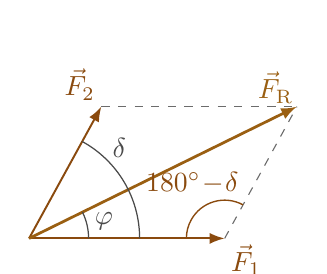
\begin{tikzpicture}[scale=1.08]
  \draw[vec] (0,0)--(2.30,0) node[below right,inner sep=2pt]{$\vec F_1$};
  \draw[vec] (0,0)--(0.85,1.55) node[above left,inner sep=2pt]{$\vec F_2$};
  \draw[hilf] (2.30,0)--(3.15,1.55);
  \draw[hilf] (0.85,1.55)--(3.15,1.55);
  \draw[bernm,line width=1pt,-{Latex[length=2mm]}] (0,0)--(3.15,1.55);
  \node[bernm,above,inner sep=2pt] at (2.90,1.52) {$\vec F_{\mathrm{R}}$};
  % phi zwischen F1 und FR
  \draw[grau,line width=0.45pt] (0.70,0) arc (0:26.2:0.70);
  \node[grau] at (0.88,0.20) {$\varphi$};
  % delta zwischen F1 und F2
  \draw[grau,line width=0.45pt] (1.30,0) arc (0:61.3:1.30);
  \node[grau] at (1.06,1.06) {$\delta$};
  % Innenwinkel des Kraeftedreiecks am Ende von F1
  \draw[bern,line width=0.5pt] ($(2.30,0)+(61.3:0.45)$) arc (61.3:180:0.45);
  \node[bern] at (1.92,0.65) {$180^\circ\!-\!\delta$};
\end{tikzpicture}
\fcap{Resultierende als Parallelogramm-Diagonale}
\par}
\hinweisD{Sonderfälle:}
\[ \begin{array}{@{}l@{\ \ }l@{}}
   \delta = 0^\circ   & F_{\mathrm{R}} = F_1 + F_2\\[0.7ex]
   \delta = 90^\circ  & F_{\mathrm{R}} = \sqrt{F_1^{\,2}+F_2^{\,2}}\\[0.7ex]
   \delta = 180^\circ & F_{\mathrm{R}} = |F_1 - F_2|
   \end{array} \]
\hinweis{Vektoren werden \emph{nie} einfach als Zahlen addiert.}
\end{minipage}
\par\vspace{1.6mm}

\TG[https://go4exercises.github.io/TALS-Physik/themen/p0-1-vorwissen-mathematik.html]{0.6}{Potenzen, Zehnerpotenzen und Vorsätze}\needspace{4\baselineskip}\ftitelD{Potenzgesetze}
\[ a^m\cdot a^n = a^{m+n}\qquad \frac{a^m}{a^n}=a^{m-n}\qquad (a^m)^n = a^{m\cdot n}\qquad a^{-n}=\frac{1}{a^n}\qquad a^0=1 \]

\begin{minipage}[t]{0.49\linewidth}\vspace{0pt}
\ftitelD{Wissenschaftliche und Engineering-Schreibweise}
\[ x = m\cdot 10^{\,n} \]
\hinweis{\(m\) Mantisse, \(n\) ganzzahliger Exponent. Die beiden Schreibweisen unterscheiden sich im
zugelassenen \emph{Mantissenbereich}:}
\[ 1\le|m|<10 \anm{wissenschaftlich} \]
\[ 1\le|m|<1000 \anm{Engineering} \]
\hinweis{In der Engineering-Form ist \(n\) zusätzlich ein \emph{Vielfaches von 3} -- das passt direkt zu den
SI-Vorsätzen.}
\end{minipage}\hfill
\begin{minipage}[t]{0.49\linewidth}\vspace{0pt}
\ftitel{Rechnen mit Zehnerpotenzen}
\hinweis{\textbf{Multiplizieren:} Mantissen multiplizieren, Exponenten \emph{addieren}.}
\hinweis{\textbf{Dividieren:} Mantissen dividieren, Exponenten \emph{subtrahieren}. Danach normieren --
je nach gewünschter Schreibweise auf \(1\le|m|<10\) (wissenschaftlich) oder \(1\le|m|<1000\) (Engineering).}
\hinweis{\textbf{Addieren und Subtrahieren:} zuerst beide Zahlen auf denselben Exponenten bringen,
dann nur die Mantissen addieren.}
\end{minipage}
\par\vspace{1.6mm}

\ftitel{SI-Vorsätze}
{\footnotesize
\setlength{\tabcolsep}{4pt}\renewcommand{\arraystretch}{1.05}
\begin{tabular}[t]{@{}l c c @{\qquad} l c c@{}}
\rowcolor{bernl} Vorsatz & Zeichen & Faktor & Vorsatz & Zeichen & Faktor\\
Tera & T & \(10^{12}\) & Dezi & d & \(10^{-1}\)\\
Giga & G & \(10^{9}\) & Zenti & c & \(10^{-2}\)\\
Mega & M & \(10^{6}\) & Milli & m & \(10^{-3}\)\\
Kilo & k & \(10^{3}\) & Mikro & \(\mu\) & \(10^{-6}\)\\
Hekto & h & \(10^{2}\) & Nano & n & \(10^{-9}\)\\
& & & Piko & p & \(10^{-12}\)\\
\end{tabular}}

\TG[https://go4exercises.github.io/TALS-Physik/themen/p0-1-vorwissen-mathematik.html]{0.7}{Gleichungen umstellen}\needspace{4\baselineskip}\ftitel{Waage-Prinzip}
\hinweis{Man formt beide Seiten gleich um -- eine \textbf{Äquivalenzumformung}: \(+\,x\), \(-\,x\), \(\cdot\,x\), \(:\,x\) (mit \(x\neq 0\)),
Quadrieren, Wurzelziehen. Der Wahrheitsgehalt der Gleichung bleibt dabei erhalten; Ziel ist, die gesuchte Grösse allein auf eine Seite zu bringen.}
\warnD{Quadrieren ist nur dann eine Äquivalenzumformung, wenn beide Seiten dasselbe Vorzeichen haben.
Einheitenkontrolle: steht links Meter, muss rechts ebenfalls Meter herauskommen.}
\[ v = \frac{s}{t}\ \ \xrightarrow{\ \cdot\,t\ }\ \ s = v\cdot t
   \ \ \xrightarrow{\ :\,v\ }\ \ t = \frac{s}{v} \]
\[ V = \pi r^{\,2} h \ \ \xrightarrow{\ :\,(\pi h)\ }\ \ r^{\,2}=\frac{V}{\pi h}
   \ \ \xrightarrow{\ \sqrt{\phantom{x}}\ }\ \ r=\sqrt{\frac{V}{\pi h}} \]
\hinweis{Erst symbolisch umstellen, dann Zahlen einsetzen -- so bleiben Rundungsfehler klein und der Rechenweg prüfbar.}

\TG[https://go4exercises.github.io/TALS-Physik/themen/p0-1-vorwissen-mathematik.html]{0.8}{Genauigkeit, Runden und Einheiten}

\begin{minipage}[t]{0.48\linewidth}\vspace{0pt}
\ftitel{Signifikante Stellen}
\hinweis{Alle Ziffern ab der ersten von null verschiedenen zählen. Führende Nullen zählen nicht,
angehängte Nullen nach dem Dezimalpunkt zählen.}
\hinweis{\textbf{Multiplikation und Division:} das Resultat erhält so viele \emph{signifikante Stellen} wie
der Faktor mit den wenigsten.\\
\textbf{Addition und Subtraktion:} das Resultat erhält so viele \emph{Dezimalstellen} wie der Summand mit den wenigsten.\\
\textbf{Exakte Zahlen} (Stückzahlen, Definitionen wie \(1\;\ME{h}=3600\;\ME{s}\)) begrenzen die Genauigkeit \emph{nicht}.}
\hinweis{\textbf{Potenzen und Wurzeln} übernehmen die signifikanten Stellen der Basis: \(v^2\) und \(\sqrt{v}\) haben so viele wie \(v\).}
\merk{\textbf{Gemischte Formeln} (Wurzeln, Potenzen, Summen und Quotienten in einem Term) lassen sich nicht Schritt für Schritt
auszählen. Praxisregel: Zwischenresultate \emph{ungerundet} weiterrechnen und das Endresultat auf so viele signifikante Stellen
runden, wie die \emph{ungenaueste Eingangsgrösse} hat -- in der Physik meist 3. Enthält der Term eine Summe oder Differenz von
Grössen sehr unterschiedlicher Genauigkeit, entscheidet diese Summe, denn dort gilt die Dezimalstellen-Regel.}

\end{minipage}\hfill
\begin{minipage}[t]{0.48\linewidth}\vspace{0pt}
\ftitel{Rundungsregel}
\hinweis{Ziffer 0--4 abrunden, 5--9 aufrunden. Zwischenresultate ungerundet weiterrechnen, erst das Endresultat runden.}
\ftitelD{Wichtige Umrechnungen}
\[ \begin{array}{@{}l@{\qquad}l@{}}
   1\;\dfrac{\ME{km}}{\ME{h}} = \dfrac{1}{3.6}\;\dfrac{\ME{m}}{\ME{s}} &
   \ME{km/h}\ \xrightarrow{\,:\,3.6\,}\ \ME{m/s}\\[2.2ex]
   1\;\ME{m^2} = 10^{4}\;\ME{cm^2} & 1\;\ME{m^3} = 10^{6}\;\ME{cm^3} = 1000\;\ME{l}\\[1.1ex]
   1\;\ME{t} = 1000\;\ME{kg} & 1\;\ME{h} = 3600\;\ME{s}\\[1.1ex]
   1\;\ME{bar} = 10^{5}\;\ME{Pa} & 1\;\ME{kWh} = 3.6\;\ME{MJ}\\[1.1ex]
   1\;\ME{Nm} = 1\;\ME{J} = 1\;\ME{Ws} & 1\;\ME{m/s^2} = 1\;\ME{N/kg}
   \end{array} \]
\warnD{Bei \emph{Arbeit und Energie} gilt \(1\;\ME{N\,m} = 1\;\ME{J}\). \emph{Drehmomente} werden trotz gleicher
Dimension in \(\ME{N\,m}\) angegeben, nicht in Joule.}
\end{minipage}

% ======================================================================
\addtocontents{toc}{\protect\columnbreak}
\LG{4}{Mechanik}\TG[https://go4exercises.github.io/TALS-Physik/themen/p4-1-kinematik.html]{4.1}{Kinematik des Schwerpunkts}\begin{minipage}[t]{0.54\linewidth}\vspace{0pt}
\ftitelD{Geschwindigkeit und Beschleunigung}
\[ \bar v = \frac{\Delta s}{\Delta t} \qquad\qquad \bar a = \frac{\Delta v}{\Delta t} \]
\hinweis{\(\Delta s\) ist die \emph{vorzeichenbehaftete} Ortsänderung. Bei Richtungsumkehr ist die tatsächlich
zurückgelegte Strecke grösser als \(|\Delta s|\).}
\hinweis{Der Querstrich kennzeichnet \textbf{Mittelwerte} über ein endliches Intervall \(\Delta t\).
Die \textbf{Momentangeschwindigkeit} \(v\) ist der Wert zu einem Zeitpunkt -- im \(s\)-\(t\)-Diagramm die Steigung der Tangente,
im Grenzfall sehr kleiner \(\Delta t\).}
\hinweis{\(1\;\ME{m/s}=3.6\;\ME{km/h}\). Bremsen ist eine Beschleunigung mit \(a<0\) (Richtung gegen \(\vec v\)).}
\end{minipage}\hfill
\begin{minipage}[t]{0.44\linewidth}\vspace{0pt}
\begin{leg}
\bar v & mittlere Geschwindigkeit & m/s\\
\Delta s & Ortsänderung entlang der Bewegungsachse & m\\
\Delta t & benötigte Zeit & s\\
\bar a & mittlere Beschleunigung & m/s\(^2\)\\
\Delta v & Geschwindigkeitsänderung & m/s
\end{leg}
\end{minipage}
\par\vspace{1.6mm}

\begin{minipage}[t]{0.54\linewidth}\vspace{0pt}
\ftitelD{Geradlinig gleichförmige Bewegung \ (\(a=0\))}
\[ s(t) = s_0 + v\cdot t\qquad v=\mtxt{konst.} \]
\end{minipage}\hfill
\begin{minipage}[t]{0.44\linewidth}\vspace{0pt}
\begin{leg}
s_0 & Anfangsposition (bei \(t=0\)) & m\\
v & konstante Geschwindigkeit & m/s
\end{leg}
{\centering\tikzfont
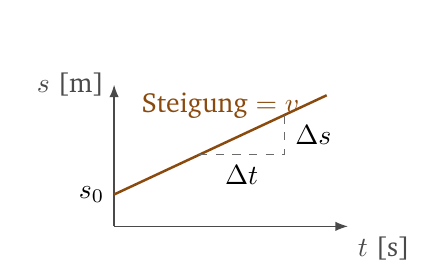
\begin{tikzpicture}[scale=0.9]
  \draw[ax] (0,0)--(3.3,0) node[below right]{$t$ [s]};
  \draw[ax] (0,0)--(0,2.0) node[left]{$s$ [m]};
  \draw[kurve] (0,0.45)--(3.0,1.85);
  \draw[hilf] (1.2,1.01)--(2.4,1.01)--(2.4,1.57);
  \node[right] at (2.42,1.29) {$\Delta s$};
  \node[below] at (1.8,0.99) {$\Delta t$};
  \node[left] at (0,0.45) {$s_0$};
  \node[bern] at (1.5,1.7) {Steigung $=v$};
\end{tikzpicture}
\fcap{gleichförmig: \(s\)-\(t\)-Diagramm}
\par}
\end{minipage}
\par\vspace{1.6mm}

\begin{minipage}[t]{0.54\linewidth}\vspace{0pt}
\ftitelD{Gleichmässig beschleunigte Bewegung \ (\(a=\text{konst.}\))}
\[ v(t) = v_0 + a\cdot t \qquad s(t) = s_0 + v_0\, t + \tfrac{1}{2}\,a\,t^{\,2} \]
\[ v^{\,2} = v_0^{\,2} + 2\,a\,(s-s_0) \anm{(zeitfrei)} \]
\hinweis{Die zeitfreie Form ist der Standardweg für Brems- und Anlaufwege ohne Zeitangabe.}
\end{minipage}\hfill
\begin{minipage}[t]{0.44\linewidth}\vspace{0pt}
\begin{leg}
v_0 & Anfangsgeschwindigkeit & m/s\\
a & konstante Beschleunigung & m/s\(^2\)
\end{leg}
{\centering\tikzfont
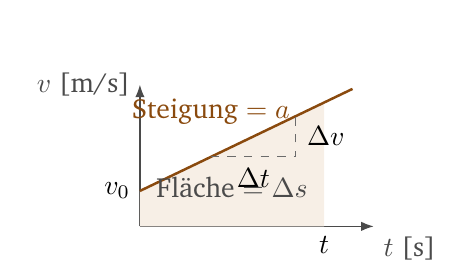
\begin{tikzpicture}[scale=0.9]
  \draw[ax] (0,0)--(3.3,0) node[below right]{$t$ [s]};
  \draw[ax] (0,0)--(0,2.0) node[left]{$v$ [m/s]};
  \fill[bernl] (0,0)--(0,0.5)--(2.6,1.75)--(2.6,0)--cycle;
  \draw[kurve] (0,0.5)--(3.0,1.94);
  \node[left] at (0,0.5) {$v_0$};
  \node[bern] at (1.0,1.62) {Steigung $=a$};
  \draw[hilf] (1.0,0.98)--(2.2,0.98)--(2.2,1.556);
  \node[below] at (1.6,0.96) {$\Delta t$};
  \node[right] at (2.22,1.27) {$\Delta v$};
  \node[grau] at (1.3,0.55) {Fläche $=\Delta s$};
  \node[below] at (2.6,0) {$t$};
\end{tikzpicture}
\fcap{beschleunigt: \(v\)-\(t\)-Diagramm}
\par}
\end{minipage}
\par\vspace{1.6mm}

\begin{minipage}[t]{0.54\linewidth}\vspace{0pt}
\ftitelD{Freier Fall (ohne Luftwiderstand)}
\[ v(t) = g\cdot t\qquad h(t)=\tfrac{1}{2}\,g\,t^{\,2} \]
\[ t = \sqrt{\frac{2h}{g}}\qquad v = \sqrt{2\,g\,h} \]
\gilt{Start aus der Ruhe (\(v_0=0\)), ohne Luftwiderstand.}
\hinweis{Die Fallzeit ist \emph{massenunabhängig}: Feder und Stein fallen im Vakuum gleich schnell.
Mit Anfangsgeschwindigkeit gelten die allgemeinen Formeln oben mit \(a=g\).}
\end{minipage}\hfill
\begin{minipage}[t]{0.44\linewidth}\vspace{0pt}
\begin{leg}
h & Fallhöhe & m\\
g & Fallbeschleunigung \(9.81\;\ME{m/s^2}\) & m/s\(^2\)\\
t & Fallzeit & s
\end{leg}
\end{minipage}
\par\vspace{1.6mm}

\begin{minipage}[t]{0.54\linewidth}\vspace{0pt}
\ftitelD{Schiefer Wurf (Wurf mit \(v_0\) unter dem Winkel \(\alpha\))}
\[ x(t) = v_0\cos\alpha\cdot t \qquad y(t) = v_0\sin\alpha\cdot t - \tfrac{1}{2}\,g\,t^{\,2} \]
\[ t_{\mathrm{F}} = \frac{2\,v_0\sin\alpha}{g}\qquad
   s_x = \frac{v_0^{\,2}\sin(2\alpha)}{g}\qquad
   h_{\max} = \frac{(v_0\sin\alpha)^2}{2g} \]
\gilt{ohne Luftwiderstand; Abwurf- und Landehöhe gleich.}
\hinweis{Überlagerung: waagrecht gleichförmig, senkrecht freier Fall.
Nur unter diesen Bedingungen ist die Wurfweite bei \(\alpha=45^\circ\) maximal.}
\end{minipage}\hfill
\begin{minipage}[t]{0.44\linewidth}\vspace{0pt}
\begin{leg}
v_0 & Abwurfgeschwindigkeit & m/s\\
\alpha & Abwurfwinkel & \(^\circ\)\\
t_{\mathrm{F}} & Flugdauer (gleiche Höhe) & s\\
s_x & Wurfweite & m\\
h_{\max} & Steighöhe & m
\end{leg}
{\centering\tikzfont
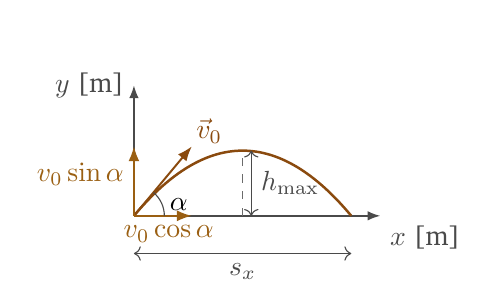
\begin{tikzpicture}[scale=0.92]
  \draw[ax] (0,0)--(3.4,0) node[below right]{$x$ [m]};
  \draw[ax] (0,0)--(0,1.8) node[left]{$y$ [m]};
  \draw[kurve,domain=0:3.0,samples=70,variable=\x] plot ({\x},{1.2*\x-0.4*\x*\x});
  \draw[vec] (0,0)--(0.80,0.96) node[above right,pos=0.9]{$\vec v_0$};
  \draw[vecg] (0,0)--(0.80,0) node[below,pos=0.6]{$v_0\cos\alpha$};
  \draw[vecg] (0,0)--(0,0.96) node[left,pos=0.6]{$v_0\sin\alpha$};
  \draw[grau,line width=0.4pt] (0.42,0) arc (0:50:0.42);
  \node at (0.62,0.16) {$\alpha$};
  \draw[hilf] (1.5,0)--(1.5,0.9);
  \draw[<->,grau,line width=0.4pt] (1.62,0)--(1.62,0.9) node[midway,right]{$h_{\max}$};
  \draw[<->,grau,line width=0.4pt] (0,-0.52)--(3.0,-0.52) node[midway,below]{$s_x$};
\end{tikzpicture}
\fcap{Wurfparabel, parametrisiert}
\par}
\end{minipage}
\par\vspace{1.6mm}

\begin{minipage}[t]{0.54\linewidth}\vspace{0pt}
\ftitelD{Gleichförmige Kreisbewegung}
\[ f = \frac{1}{T}\qquad \omega = \frac{2\pi}{T} = 2\pi f\qquad v = \omega\cdot r \]
\[ a_{\mathrm{z}} = \frac{v^{\,2}}{r} = \omega^{\,2}\cdot r \qquad F_{\mathrm{z}} = m\cdot a_{\mathrm{z}} = \frac{m\,v^{\,2}}{r} \]
\hinweis{Der Betrag von \(\vec v\) ist konstant, die \emph{Richtung} ändert sich -- deshalb ist die Kreisbewegung beschleunigt.}
\end{minipage}\hfill
\begin{minipage}[t]{0.44\linewidth}\vspace{0pt}
\begin{leg}
T & Umlaufdauer (Periode) & s\\
f & Drehfrequenz & Hz \(=1/\)s\\
\omega & Winkelgeschwindigkeit & rad/s\\
r & Bahnradius & m\\
a_{\mathrm{z}} & Zentripetalbeschleunigung & m/s\(^2\)\\
F_{\mathrm{z}} & Zentripetalkraft (zum Zentrum) & N
\end{leg}
{\centering\tikzfont
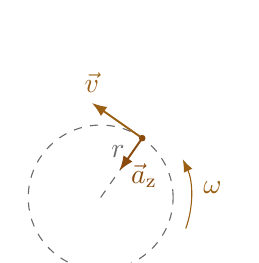
\begin{tikzpicture}[scale=0.92]
  \draw[hilf] (0,0) circle (1.0);
  \coordinate (P) at (55:1.0);
  \draw[hilf] (0,0)--(P);
  \node[hgrau] at (0.24,0.64) {$r$};
  \draw[vecg] (P)--($(P)+(145:0.85)$) node[above,pos=1.0]{$\vec v$};
  \draw[vec] (P)--($(P)+(235:0.55)$);
  \node[bern] at (0.60,0.30) {$\vec a_{\mathrm{z}}$};
  \fill[bern] (P) circle (1.3pt);
  \draw[bernm,-{Latex[length=1.6mm]}] (-20:1.25) arc (-20:25:1.25);
  \node[bernm] at (5:1.55) {$\omega$};
\end{tikzpicture}
\fcap{\(\vec v\) tangential, \(\vec a_{\mathrm{z}}\) zum Zentrum}
\par}
\end{minipage}
\par\vspace{1.6mm}

\begin{minipage}[t]{0.54\linewidth}\vspace{0pt}
\ftitelD{Zusammengesetzte Bewegung}
\[ \vec v_{\text{res}} = \vec v_1 + \vec v_2 \]
\hinweis{Beispielmuster Schwimmer/Strömung, Flugzeug/Wind: senkrechte Anteile mit
\(v_{\text{res}}=\sqrt{v_1^{\,2}+v_2^{\,2}}\) (siehe \(\S\,0.5\)). Die Teilbewegungen sind voneinander unabhängig.}
\end{minipage}\hfill
\begin{minipage}[t]{0.44\linewidth}\vspace{0pt}
\begin{leg}
\vec v_{\text{res}} & resultierende Geschwindigkeit & m/s\\
\vec v_1,\vec v_2 & Teilgeschwindigkeiten & m/s
\end{leg}
{\centering\tikzfont
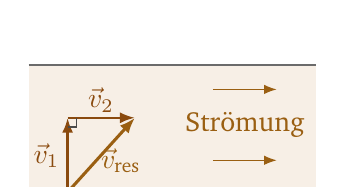
\begin{tikzpicture}[scale=0.90]
  % Fluss
  \fill[bernl] (0,0) rectangle (4.05,1.80);
  \draw[hgrau,line width=0.7pt] (0,0)--(4.05,0);
  \draw[hgrau,line width=0.7pt] (0,1.80)--(4.05,1.80);
  % Stroemung
  \draw[bernm,-{Latex[length=1.6mm]}] (2.60,0.45)--(3.50,0.45);
  \draw[bernm,-{Latex[length=1.6mm]}] (2.60,1.45)--(3.50,1.45);
  \node[bernm] at (3.05,0.95) {Strömung};
  % Vektordreieck: v1 + v2 = v_res  (schliesst exakt)
  \draw[vec,line width=0.9pt] (0.55,0)--(0.55,1.05);
  \node[bern,left,inner sep=2pt] at (0.52,0.52) {$\vec v_1$};
  \draw[vec,line width=0.9pt] (0.55,1.05)--(1.50,1.05);
  \node[bern] at (1.02,1.30) {$\vec v_2$};
  \draw[bernm,line width=1.1pt,-{Latex[length=2mm]}] (0.55,0)--(1.50,1.05);
  \node[bernm] at (1.30,0.45) {$\vec v_{\text{res}}$};
  % rechter Winkel zwischen v1 und v2
  \draw[grau,line width=0.4pt] (0.55,0.92)--(0.68,0.92)--(0.68,1.05);
  \fill[bern] (0.55,0) circle (1.2pt);
\end{tikzpicture}
\fcap{Schwimmer quer zur Strömung: die Teilbewegungen überlagern sich}
\par}
\end{minipage}
\par\vspace{1.6mm}

\TG[https://go4exercises.github.io/TALS-Physik/themen/p4-2-dynamik.html]{4.2}{Dynamik}\begin{minipage}[t]{0.54\linewidth}\vspace{0pt}
\ftitelD{Newtonsche Gesetze}
\[ \begin{array}{@{}r@{\ \ }l@{\quad}l@{}}
   \textbf{1.} & \vec F_{\text{ges}} = \vec 0 \ \Rightarrow\ \vec v = \mtxt{konstant} & \anm{Trägheitsgesetz}\\[0.9ex]
   \textbf{2.} & \vec F_{\text{ges}} = m\cdot\vec a & \anm{Grundgesetz der Dynamik}\\[0.9ex]
   \textbf{3.} & \vec F_{12} = -\,\vec F_{21} & \anm{actio \(=\) reactio}
   \end{array} \]
\warnD{Die beiden Kräfte des dritten Gesetzes wirken gleichzeitig auf \emph{verschiedene} Körper und dürfen
deshalb nicht im selben Freikörperbild gegeneinander gekürzt werden.}
\end{minipage}\hfill
\begin{minipage}[t]{0.44\linewidth}\vspace{0pt}
\begin{leg}
\vec F_{\text{ges}} & resultierende Kraft & N \(=\ME{kg\,m/s^2}\)\\
m & Masse & kg\\
\vec a & Beschleunigung & m/s\(^2\)
\end{leg}
\end{minipage}
\par\vspace{1.6mm}

\begin{minipage}[t]{0.54\linewidth}\vspace{0pt}
\ftitelD{Gewichtskraft}
\[ F_{\mathrm{G}} = m\cdot g \]
\hinweis{Beide Schreibweisen sind gleichwertig: \(9.81\;\ME{m/s^2} = 9.81\;\ME{N/kg}\).
In \emph{dynamischen} Aufgaben (Fall, Beschleunigung) rechnet man mit \(\ME{m/s^2}\); in \emph{statischen}
Aufgaben (Gewichtskraft, Auflagerkräfte) ist \(\ME{N/kg}\) anschaulicher -- je Kilogramm Masse wirken \(9.81\;\ME{N}\).}
\hinweis{Masse ist ortsunabhängig, die Gewichtskraft nicht (Mond: \(g\approx 1.62\;\ME{m/s^2}\)).}
\end{minipage}\hfill
\begin{minipage}[t]{0.44\linewidth}\vspace{0pt}
\begin{leg}
F_{\mathrm{G}} & Gewichtskraft & N\\
g & Ortsfaktor, Erde \(9.81\) & m/s\(^2\) bzw.\ N/kg
\end{leg}
\end{minipage}
\par\vspace{1.6mm}

\begin{minipage}[t]{0.54\linewidth}\vspace{0pt}
\ftitelD{Federkraft (Hookesches Gesetz)}
\[ F = D\cdot s \]
\gilt{elastischer Bereich, bis zur Proportionalitätsgrenze der Feder.}
\end{minipage}\hfill
\begin{minipage}[t]{0.44\linewidth}\vspace{0pt}
\begin{leg}
D & Federkonstante & N/m\\
s & Verlängerung / Stauchung & m
\end{leg}
{\centering\tikzfont
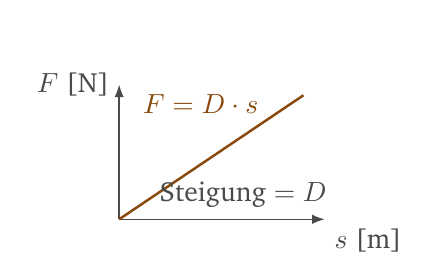
\begin{tikzpicture}[scale=0.9]
  \draw[ax] (0,0)--(2.9,0) node[below right]{$s$ [m]};
  \draw[ax] (0,0)--(0,1.9) node[left]{$F$ [N]};
  \draw[kurve] (0,0)--(2.6,1.75);
  \node[bern] at (1.15,1.62) {$F=D\cdot s$};
  \node[grau] at (1.75,0.35) {Steigung $=D$};
\end{tikzpicture}
\fcap{Federkennlinie}
\par}
\end{minipage}
\par\vspace{1.6mm}

\begin{minipage}[t]{0.54\linewidth}\vspace{0pt}
\ftitelD{Reibungskraft}
\[ \mtxt{Gleiten:}\quad F_{\mathrm{R}} = \mu_{\text{G}}\cdot F_{\mathrm{N}} \]
\[ \mtxt{Haften:}\quad F_{\mathrm{R}} \le \mu_{\text{H}}\cdot F_{\mathrm{N}}
   \qquad F_{\mathrm{R,max}} = \mu_{\text{H}}\cdot F_{\mathrm{N}} \]
\hinweis{Beim \emph{Gleiten} ist \(F_{\mathrm{R}}\) festgelegt. Beim \emph{Haften} passt sich die Reibungskraft der
angreifenden Kraft an -- bis zum Maximalwert \(F_{\mathrm{R,max}}\); erst darüber setzt Bewegung ein.
Nur diesen Maximalwert einsetzen, wenn nach dem Losbrechen gefragt ist. Meist gilt \(\mu_{\text{H}} \ge \mu_{\text{G}}\).}
\gilt{vereinfachtes Coulomb-Reibungsmodell -- nur darin ist \(F_{\mathrm{R}}\) unabhängig von der Kontaktfläche.}
\end{minipage}\hfill
\begin{minipage}[t]{0.44\linewidth}\vspace{0pt}
\begin{leg}
F_{\mathrm{R}} & Reibungskraft & N\\
\mu_{\text{H}},\mu_{\text{G}} & Haft- und Gleitreibungszahl & --\\
F_{\mathrm{N}} & Normalkraft (senkrecht zur Fläche) & N
\end{leg}
\end{minipage}
\par\vspace{1.6mm}

\begin{minipage}[t]{0.54\linewidth}\vspace{0pt}
\ftitelD{Schiefe Ebene}
\[ F_{\mathrm{H}} = F_{\mathrm{G}}\sin\alpha = m\,g\,\sin\alpha \qquad
   F_{\mathrm{N}} = F_{\mathrm{G}}\cos\alpha = m\,g\,\cos\alpha \]
\[ \begin{array}{@{}l@{\quad}l@{}}
   \textbf{Gleiten:} & F_{\mathrm{R}} = \mu_{\text{G}}\,F_{\mathrm{N}} = \mu_{\text{G}}\,m\,g\,\cos\alpha\\[0.8ex]
   \textbf{Haften:}  & 0 \le F_{\mathrm{R}} \le \mu_{\text{H}}\,F_{\mathrm{N}},
                       \quad F_{\mathrm{R,max}} = \mu_{\text{H}}\,F_{\mathrm{N}}
   \end{array} \]
\zwiD{\textbf{Grundgleichung} längs der Ebene (2. Newtonsches Gesetz):}
\[ m\cdot a = F_{\mathrm{H}} - F_{\mathrm{R}} \]
\zwiD{\textbf{Fallunterscheidung} -- verglichen wird mit der maximalen Haftreibung
\(F_{\mathrm{R,max}} = \mu_{\text{H}}\,F_{\mathrm{N}}\):}
\[ \begin{array}{@{}l@{\quad}l@{\quad}l@{}}
   F_{\mathrm{H}} < F_{\mathrm{R,max}} & a = 0,\quad F_{\mathrm{R}} = F_{\mathrm{H}}
     & \anm{statisch: Körper bleibt liegen}\\[0.8ex]
   F_{\mathrm{H}} = F_{\mathrm{R,max}} & a = 0,\quad \tan\alpha = \mu_{\text{H}}
     & \anm{Übergang: Losbrechen}\\[0.8ex]
   F_{\mathrm{H}} > F_{\mathrm{R,max}} & F_{\mathrm{R}} = \mu_{\text{G}}\,F_{\mathrm{N}}
     & \anm{dynamisch: Körper gleitet}
   \end{array} \]
\zwiD{Im Gleitfall eingesetzt -- die Masse kürzt sich heraus:}
\[ a = g\,(\sin\alpha - \mu_{\text{G}}\cdot\cos\alpha) \]
\gilt{vereinfachtes Reibungsmodell; \(a\) gilt für den hangabwärts gleitenden Körper.}
\hinweis{Im statischen Fall passt sich \(F_{\mathrm{R}}\) an \(F_{\mathrm{H}}\) an -- nicht \(\mu_{\text{H}}F_{\mathrm{N}}\) einsetzen!
Der \emph{Grenzwinkel} folgt aus dem Übergangsfall: \(\alpha_{\max} = \arctan\mu_{\text{H}}\).
Gleitet der Körper \emph{hangaufwärts}, wirkt die Reibung ebenfalls hangabwärts:
\(a = -g\,(\sin\alpha + \mu_{\text{G}}\cos\alpha)\).}
\end{minipage}\hfill
\begin{minipage}[t]{0.44\linewidth}\vspace{0pt}
\begin{leg}
F_{\mathrm{H}} & Hangabtriebskraft (parallel zur Ebene) & N\\
F_{\mathrm{N}} & Normalkraft (senkrecht zur Ebene) & N\\
F_{\mathrm{G},\perp} & Komponente von \(F_{\mathrm{G}}\) senkrecht zur Ebene & N\\
F_{\mathrm{R}} & Reibungskraft (entgegen der Bewegung) & N\\
\mu_{\text{H}},\mu_{\text{G}} & Haft- und Gleitreibungszahl & --\\
\alpha & Neigungswinkel & \(^\circ\)\\
a & Beschleunigung hangabwärts & m/s\(^2\)
\end{leg}
{\centering\tikzfont
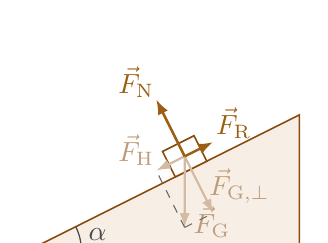
\begin{tikzpicture}[scale=0.86]
  \draw[koerper,fill=bernl] (0,0)--(4.00,0)--(4.00,2.00)--cycle;
  \draw[grau,line width=0.45pt] (0.78,0) arc (0:26.57:0.78);
  \node[grau] at (1.02,0.24) {$\alpha$};
  \coordinate (P) at (2.40,1.20);
  \coordinate (C) at (2.306,1.388);
  \draw[koerper,fill=white,rotate around={26.57:(P)}] ($(P)+(-0.26,0)$) rectangle ($(P)+(0.26,0.42)$);
  % --- Ursache und ihre Komponenten: matt ---
  \draw[-{Latex[length=1.8mm,width=1.3mm]},bern!38,line width=0.8pt] (C)--(2.306,0.338);
  \node[bern!55,right,inner sep=2pt] at (2.35,0.42) {$\vec F_{\mathrm{G}}$};
  \draw[-{Latex[length=1.8mm,width=1.3mm]},bern!38,line width=0.8pt] (C)--(1.886,1.178);
  \node[bern!55,above left,inner sep=1pt] at (1.90,1.20) {$\vec F_{\mathrm{H}}$};
  \draw[-{Latex[length=1.8mm,width=1.3mm]},bern!38,line width=0.8pt] (C)--(2.726,0.548);
  \node[bern!55,right,inner sep=2pt] at (2.58,0.95) {$\vec F_{\mathrm{G},\perp}$};
  \draw[hilf] (2.306,0.338)--(1.886,1.178);
  \draw[hilf] (2.306,0.338)--(2.726,0.548);
  % --- Gegenkräfte: kräftig ---
  \draw[vecg,line width=0.9pt] (C)--(1.886,2.228);
  \node[bernm,above left,inner sep=1pt] at (1.90,2.21) {$\vec F_{\mathrm{N}}$};
  \draw[vecg,line width=0.9pt] (C)--(2.726,1.598);
  \node[bernm,above right,inner sep=1pt] at (2.72,1.60) {$\vec F_{\mathrm{R}}$};
\end{tikzpicture}
\fcap{matt: Ursache \(\vec F_{\mathrm{G}}\) und ihre Komponenten -- kräftig: die beiden Gegenkräfte}
\par}
\hinweis{\textbf{Zur Skizze:} \(\vec F_{\mathrm{G}}\) ist die \emph{Ursache} und deshalb matt gezeichnet.
Sie zerfällt in \(\vec F_{\mathrm{H}}\) längs der Ebene und \(\vec F_{\mathrm{G},\perp}\) senkrecht dazu.
Kräftig gezeichnet sind die beiden \emph{Gegenkräfte}: \(\vec F_{\mathrm{N}}\) hebt \(\vec F_{\mathrm{G},\perp}\) auf
(die Unterlage drückt zurück, \(F_{\mathrm{N}} = F_{\mathrm{G},\perp}\)), \(\vec F_{\mathrm{R}}\) wirkt \(\vec F_{\mathrm{H}}\) entgegen.
Übrig bleibt längs der Ebene \(F_{\mathrm{H}} - F_{\mathrm{R}}\) -- genau die Grundgleichung.}
\warnD{\(\vec F_{\mathrm{G}}\) und seine Komponenten \(\vec F_{\mathrm{H}}\), \(\vec F_{\mathrm{G},\perp}\) niemals
gleichzeitig in derselben Kraftsumme verwenden -- entweder die Gewichtskraft oder ihre Zerlegung.}
\end{minipage}
\par\vspace{1.6mm}

\begin{minipage}[t]{0.54\linewidth}\vspace{0pt}
\ftitelD{Zwei Massen an einem Faden (Atwood)}
\[ a = \frac{(m_1-m_2)\,g}{m_1+m_2}\qquad F_{\mathrm{S}} = \frac{2\,m_1 m_2\,g}{m_1+m_2} \]
\gilt{masseloses, undehnbares Seil; reibungsfreie, masselose Rolle.}
\end{minipage}\hfill
\begin{minipage}[t]{0.44\linewidth}\vspace{0pt}
\begin{leg}
m_1,m_2 & Massen (\(m_1>m_2\)) & kg\\
F_{\mathrm{S}} & Fadenkraft & N
\end{leg}
{\centering\tikzfont
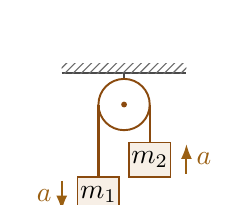
\begin{tikzpicture}[scale=0.88]
  \draw[grau,line width=0.7pt] (0.30,2.60)--(2.10,2.60);
  \fill[pattern=north east lines,pattern color=hgrau] (0.30,2.60) rectangle (2.10,2.74);
  \draw[grau,line width=0.6pt] (1.20,2.52)--(1.20,2.60);
  \draw[koerper,fill=white,line width=0.7pt] (1.20,2.15) circle (0.37);
  \fill[bern] (1.20,2.15) circle (1.2pt);
  \draw[bern,line width=0.8pt] (0.83,2.15)--(0.83,1.10);
  \draw[bern,line width=0.8pt] (1.57,2.15)--(1.57,1.60);
  \draw[koerper] (0.53,0.60) rectangle (1.13,1.10);
  \node at (0.83,0.85) {$m_1$};
  \draw[koerper] (1.27,1.10) rectangle (1.87,1.60);
  \node at (1.57,1.35) {$m_2$};
  \draw[vecg] (0.30,1.05)--(0.30,0.62) node[left,pos=0.5]{$a$};
  \draw[vecg] (2.10,1.15)--(2.10,1.58) node[right,pos=0.5]{$a$};
\end{tikzpicture}
\fcap{\(m_1>m_2\): gleicher Betrag von \(a\), entgegengesetzte Richtung}
\par}
\end{minipage}
\par\vspace{1.6mm}

\begin{minipage}[t]{0.54\linewidth}\vspace{0pt}
\ftitelD{Scheinbares Gewicht im Lift}
\[ F_{\mathrm{N}} = m\,(g \pm a) \]
\hinweisD{\(+\) bei Beschleunigung nach oben, \(-\) nach unten:}
\[ \begin{array}{@{}l@{\quad}c@{\quad}l@{}}
   \vec a \mtxt{ nach oben} & F_{\mathrm{N}} > F_{\mathrm{G}} & \anm{man fühlt sich schwerer}\\[0.7ex]
   \vec a \mtxt{ nach unten} & F_{\mathrm{N}} < F_{\mathrm{G}} & \anm{man fühlt sich leichter}\\[0.7ex]
   a = 0 & F_{\mathrm{N}} = F_{\mathrm{G}} & \anm{Stillstand oder konstante Fahrt}
   \end{array} \]
\hinweis{Entscheidend ist die Richtung der \emph{Beschleunigung}, nicht die Fahrtrichtung: ein anfahrender Abwärtslift
beschleunigt nach unten (leichter), ein bremsender Abwärtslift nach oben (schwerer).
Im freien Fall (\(a=g\)) wird \(F_{\mathrm{N}}=0\) -- Schwerelosigkeit.}
\end{minipage}\hfill
\begin{minipage}[t]{0.44\linewidth}\vspace{0pt}
\begin{leg}
F_{\mathrm{N}} & Normalkraft, Anzeige der Waage & N\\
a & Betrag der Kabinenbeschleunigung & m/s\(^2\)
\end{leg}
{\centering\tikzfont
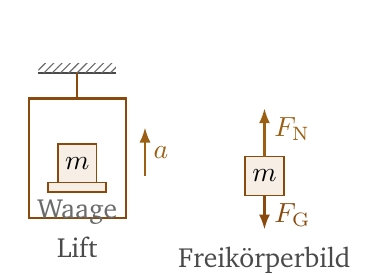
\begin{tikzpicture}[scale=0.82]
  % ===== links: Lift =====
  \draw[grau,line width=0.7pt] (0.40,2.45)--(1.60,2.45);
  \fill[pattern=north east lines,pattern color=hgrau] (0.40,2.45) rectangle (1.60,2.59);
  \draw[bern,line width=0.8pt] (1.00,2.45)--(1.00,2.05);
  \draw[koerper,fill=white,line width=0.8pt] (0.25,0.20) rectangle (1.75,2.05);
  \draw[koerper,fill=bernl] (0.55,0.60) rectangle (1.45,0.75);
  \draw[koerper] (0.70,0.75) rectangle (1.30,1.35);
  \node at (1.00,1.05) {$m$};
  \node[hgrau,below,inner sep=1.5pt] at (1.00,0.55) {Waage};
  \draw[vecg] (2.05,0.85)--(2.05,1.60);
  \node[bernm,right,inner sep=2pt] at (2.09,1.22) {$a$};
  \node[grau,below] at (1.00,0.05) {Lift};
  % ===== rechts: Freikörperbild der Masse =====
  \begin{scope}[xshift=3.30cm]
    \draw[koerper] (0.30,0.55) rectangle (0.90,1.15);
    \node at (0.60,0.85) {$m$};
    \draw[vecg,line width=0.9pt] (0.60,1.15)--(0.60,1.90);
    \node[bernm,right,inner sep=2pt] at (0.66,1.58) {$F_{\mathrm{N}}$};
    \draw[vec,line width=0.9pt] (0.60,0.55)--(0.60,0.02);
    \node[bern,right,inner sep=2pt] at (0.66,0.24) {$F_{\mathrm{G}}$};
    \node[grau,below] at (0.60,-0.10) {Freikörperbild};
  \end{scope}
\end{tikzpicture}
\fcap{Die Waage zeigt \(F_{\mathrm{N}}\) an, nicht die Gewichtskraft}
\par}
\end{minipage}
\par\vspace{1.6mm}

\TG[https://go4exercises.github.io/TALS-Physik/themen/p4-3-energie.html]{4.3}{Energie}\begin{minipage}[t]{0.54\linewidth}\vspace{0pt}
\ftitelD{Mechanische Arbeit}
\[ W = F\cdot s\cdot\cos\alpha \]
\gilt{konstante Kraft, geradlinige Verschiebung.}
\hinweis{Nur der Kraftanteil \emph{längs} des Weges verrichtet Arbeit. \(\alpha=90^\circ \Rightarrow W=0\) (Tragen auf Ebene).
Bei veränderlicher Kraft ist \(W\) die Fläche unter dem \(F\)-\(s\)-Diagramm.}
\end{minipage}\hfill
\begin{minipage}[t]{0.44\linewidth}\vspace{0pt}
\begin{leg}
W & Arbeit & J \(=\ME{Nm}\)\\
F & Betrag der Kraft & N\\
s & Weg & m\\
\alpha & Winkel zwischen \(\vec F\) und \(\vec s\) & \(^\circ\)
\end{leg}
{\centering\tikzfont
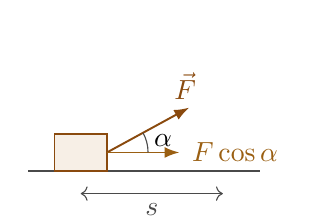
\begin{tikzpicture}[scale=0.95]
  \draw[grau,line width=0.5pt] (0,0)--(3.1,0);
  \draw[koerper] (0.35,0) rectangle (1.05,0.5);
  \draw[vec] (1.05,0.25)--(2.15,0.85) node[above,pos=0.95]{$\vec F$};
  \draw[vecg] (1.05,0.25)--(2.02,0.25);
  \node[bernm,right] at (2.06,0.25) {$F\cos\alpha$};
  \draw[grau,line width=0.4pt] (1.60,0.25) arc (0:28.6:0.55);
  \node at (1.80,0.41) {$\alpha$};
  \draw[<->,grau,line width=0.4pt] (0.7,-0.3)--(2.6,-0.3) node[midway,below]{$s$};
\end{tikzpicture}
\fcap{nur \(F\cos\alpha\) verrichtet Arbeit}
\par}
\end{minipage}
\par\vspace{1.6mm}

\begin{minipage}[t]{0.54\linewidth}\vspace{0pt}
\ftitelD{Energieformen}
\[ E_{\text{pot}} = m\,g\,h \qquad E_{\text{kin}} = \tfrac{1}{2}\,m\,v^{\,2}\qquad
   E_{\text{sp}} = \tfrac{1}{2}\,D\,s^{\,2} \]
\hinweis{\(E_{\text{kin}}\) wächst \emph{quadratisch} mit \(v\): doppeltes Tempo, vierfache Energie (Bremsweg!).}
\merk{\textbf{Energie oder Arbeit?} \(E\) ist eine \textbf{Zustandsgrösse}: sie sagt, wie viel ein Körper
\emph{gespeichert hat} (Lage, Bewegung, Spannung). \(W\) ist eine \textbf{Prozessgrösse}: sie sagt, wie viel Energie beim
Vorgang \emph{übertragen} wurde. Beide haben die Einheit Joule. Arbeit ist \emph{Energieübertragung}: die
\emph{resultierende} Arbeit an einem Körper entspricht der Änderung seiner kinetischen Energie,
\(W_{\text{res}} = \Delta E_{\text{kin}}\) (Arbeitssatz). Für ein gewähltes System kann von aussen verrichtete Arbeit
dessen Gesamtenergie verändern -- das ist aber nicht dasselbe wie die Arbeit einer beliebigen Einzelkraft.}
\end{minipage}\hfill
\begin{minipage}[t]{0.44\linewidth}\vspace{0pt}
\begin{leg}
E_{\text{pot}} & Höhenenergie & J\\
h & Höhe über frei wählbarem Nullniveau & m\\
E_{\text{kin}} & Bewegungsenergie & J\\
E_{\text{sp}} & Spannenergie der Feder & J
\end{leg}
{\centering\tikzfont
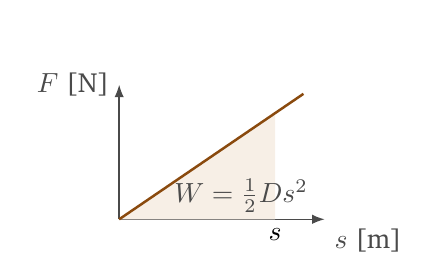
\begin{tikzpicture}[scale=0.9]
  \draw[ax] (0,0)--(2.9,0) node[below right]{$s$ [m]};
  \draw[ax] (0,0)--(0,1.9) node[left]{$F$ [N]};
  \fill[bernl] (0,0)--(2.2,1.5)--(2.2,0)--cycle;
  \draw[kurve] (0,0)--(2.6,1.77);
  \node[grau] at (1.72,0.33) {$W=\tfrac{1}{2}Ds^2$};
  \node[below] at (2.2,0) {$s$};
\end{tikzpicture}
\fcap{Spannarbeit: Federkraft wächst, Fläche \(=\) Dreieck}
\vspace{2mm}

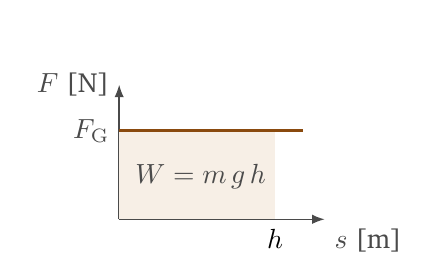
\begin{tikzpicture}[scale=0.9]
  \draw[ax] (0,0)--(2.9,0) node[below right]{$s$ [m]};
  \draw[ax] (0,0)--(0,1.9) node[left]{$F$ [N]};
  \fill[bernl] (0,0) rectangle (2.2,1.25);
  \draw[kurve] (0,1.25)--(2.6,1.25);
  \node[left,grau] at (0,1.25) {$F_{\mathrm{G}}$};
  \node[grau] at (1.15,0.60) {$W=m\,g\,h$};
  \node[below] at (2.2,0) {$h$};
\end{tikzpicture}
\fcap{Hubarbeit: Kraft konstant, Fläche \(=\) Rechteck}
\par}
\end{minipage}
\par\vspace{1.6mm}

\ftitelD{Energieerhaltung (ohne Reibung)}
\[ E_{\text{kin}} + E_{\text{pot}} + E_{\text{sp}} = \mtxt{konstant} \]
\gilt{reibungsfrei, geschlossenes System.}
\hinweis{\textbf{Bungee-Sprung} als Beispiel für alle drei Formen: oben nur \(E_{\text{pot}}\) -- im freien Fall wandelt sie
sich in \(E_{\text{kin}}\) -- beim Dehnen des Seils geht beides in \(E_{\text{sp}}\) über. Die \emph{Summe} bleibt gleich.}
\zwiD{\textbf{Spezialfall} -- Start aus der Ruhe, nur Höhenverlust \(h\), keine Feder:}
\[ m\,g\,h = \tfrac{1}{2}\,m\,v^{\,2} \qquad\Longrightarrow\qquad v = \sqrt{2\,g\,h} \]
\hinweis{Die Masse kürzt sich heraus -- die Endgeschwindigkeit ist massenunabhängig.}
\zwiD{\textbf{Beispiel schiefe Ebene} -- reibungsfrei, Start aus der Ruhe, Rutschlänge \(s\), Neigung \(\alpha\):}
\[ h = s\cdot\sin\alpha \qquad\Longrightarrow\qquad v = \sqrt{2\,g\,s\,\sin\alpha} \]
\hinweis{Nur die \emph{Höhe} zählt, nicht der zurückgelegte Weg: bei gleicher Höhe ist die Endgeschwindigkeit unabhängig
von der Neigung -- die flachere Bahn dauert nur länger. Dasselbe gilt für den freien Fall (\(\alpha = 90^\circ\)).}

\ftitelD{Energiebilanz mit Reibung}
\[ W_{\mathrm{R}} = -\,F_{\mathrm{R}}\cdot s \qquad E_{\text{diss}} = F_{\mathrm{R}}\cdot s \]
\[ E_{\text{Anfang}} = E_{\text{Ende}} + E_{\text{diss}} \]
\hinweis{Die \emph{Arbeit} der Reibungskraft \(W_{\mathrm{R}}\) ist negativ (sie wirkt gegen die Bewegung); die \emph{dissipierte Energie}
\(E_{\text{diss}}=|W_{\mathrm{R}}|\) ist positiv und erscheint als Wärme. Beide Grössen nie im selben Term mischen.}

\begin{minipage}[t]{0.54\linewidth}\vspace{0pt}
\ftitelD{Leistung}
\[ \bar P = \frac{W}{\Delta t} = \frac{\Delta E}{\Delta t} \anm{mittlere Leistung} \]
\[ P = \vec F\cdot\vec v = F\cdot v\cdot\cos\alpha \anm{momentane Leistung} \]
\[ \mtxt{bei } \vec F \parallel \vec v:\qquad P = F\cdot v \]
\hinweis{\(1\;\ME{kWh} = 3.6\;\ME{MJ}\); \(1\;\ME{PS}\approx 736\;\ME{W}\).}
\end{minipage}\hfill
\begin{minipage}[t]{0.44\linewidth}\vspace{0pt}
\begin{leg}
\bar P & mittlere Leistung über \(\Delta t\) & W \(=\ME{J/s}\)\\
P & momentane Leistung & W\\
\Delta t & Zeitintervall & s\\
v & Geschwindigkeit & m/s\\
\alpha & Winkel zwischen \(\vec F\) und \(\vec v\) & \(^\circ\)
\end{leg}
\end{minipage}
\par\vspace{1.6mm}

\begin{minipage}[t]{0.54\linewidth}\vspace{0pt}
\ftitelD{Wirkungsgrad}
\[ \eta = \frac{E_{\text{nutz}}}{E_{\text{zu}}} = \frac{P_{\text{nutz}}}{P_{\text{zu}}} \le 1
   \qquad \eta_{\text{ges}} = \eta_1\cdot\eta_2\cdot\ldots \]
\hinweis{Die Differenz \(E_{\text{zu}}-E_{\text{nutz}}\) wird in nicht nutzbare Energieformen umgewandelt --
meist in innere bzw. thermische Energie, teilweise auch in Schall oder Verformung.
Bei einer Kette werden die Wirkungsgrade \emph{multipliziert}.}
\end{minipage}\hfill
\begin{minipage}[t]{0.44\linewidth}\vspace{0pt}
\begin{leg}
\eta & Wirkungsgrad & -- (oder \%)\\
E_{\text{nutz}} & nutzbar abgegebene Energie & J\\
E_{\text{zu}} & zugeführte Energie & J
\end{leg}
\end{minipage}
\par\vspace{1.6mm}

\TG[https://go4exercises.github.io/TALS-Physik/themen/p4-4-statik.html]{4.4}{Statik von Festkörpern}\begin{minipage}[t]{0.54\linewidth}\vspace{0pt}
\ftitelD{Kräftezerlegung und Resultierende}
\[ F_x = F\cos\varphi\qquad F_y = F\sin\varphi \]
\[ \vec F_{\mathrm{R}} = \sum_i \vec F_i \]
\end{minipage}\hfill
\begin{minipage}[t]{0.44\linewidth}\vspace{0pt}
\begin{leg}
\vec F_{\mathrm{R}} & Resultierende aller Kräfte & N\\
\varphi & Winkel zur \(x\)-Achse & \(^\circ\)
\end{leg}
\end{minipage}
\par\vspace{1.6mm}

\begin{minipage}[t]{0.54\linewidth}\vspace{0pt}
\ftitelD{Drehmoment}
\[ M = F\cdot r = F\cdot l\cdot\sin\alpha \]
\hinweisD{Derselbe Term, zwei Lesarten -- beide führen zum gleichen Drehmoment:}
\[ M = F\cdot(l\,\sin\alpha) \anm{verkürzter Hebel: ganze Kraft \(\times\) Hebelarm} \]
\[ M = l\cdot(F\,\sin\alpha) \anm{verkürzte Kraft: ganzer Hebel \(\times\) Kraftanteil} \]
\hinweis{Nur der \emph{senkrecht zum Hebel} stehende Kraftanteil \(F\sin\alpha\) dreht; der Anteil längs des Hebels
zieht nur an der Drehachse. Maximal bei \(\alpha=90^\circ\) (\(M=F\,l\)), null bei \(\alpha=0^\circ\).
Drehrichtung durch das Vorzeichen unterscheiden.}
\end{minipage}\hfill
\begin{minipage}[t]{0.44\linewidth}\vspace{0pt}
\begin{leg}
M & Drehmoment & Nm\\
F & Kraft & N\\
r & Hebelarm (Abstand Drehachse--Wirkungslinie) & m\\
l & Abstand Drehachse--Angriffspunkt & m\\
\alpha & Winkel zwischen Hebel und Kraft & \(^\circ\)
\end{leg}
{\centering\tikzfont
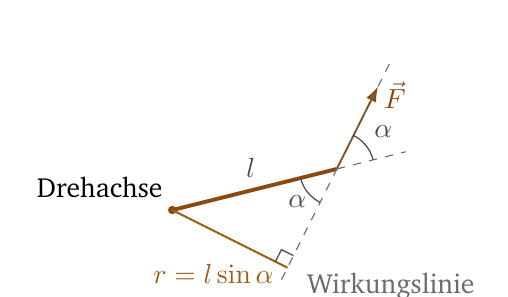
\begin{tikzpicture}[scale=0.95]
  \fill[bern] (0,0) circle (1.6pt); \node[above left] at (0,0.04) {Drehachse};
  \draw[koerper,line width=1.4pt] (0,0)--(2.2,0.55);
  \draw[vec] (2.2,0.55)--(2.75,1.65) node[right,pos=0.9]{$\vec F$};
  \draw[hilf] (2.90,1.95)--(1.45,-0.95);
  \node[hgrau,right,inner sep=2pt] at (1.72,-1.02) {Wirkungslinie};
  \draw[hilf] (2.20,0.55)--(3.12,0.78);
  \draw[grau,line width=0.45pt] ($(2.20,0.55)+(14.04:0.50)$) arc (14.04:63.43:0.50);
  \node[grau] at (2.82,1.05) {$\alpha$};
  \draw[grau,line width=0.45pt] ($(2.20,0.55)+(194.04:0.50)$) arc (194.04:243.43:0.50);
  \node[grau] at (1.67,0.12) {$\alpha$};
  \node[above,grau] at (1.05,0.30) {$l$};
  \draw[bernm,line width=0.7pt] (0,0)--(1.54,-0.77);
  \node[bernm] at (0.55,-0.85) {$r=l\sin\alpha$};
  \draw[grau,line width=0.45pt] (1.379,-0.690)--(1.459,-0.529)--(1.620,-0.609);
\end{tikzpicture}
\fcap{Hebelarm \(r\) steht senkrecht auf \(\vec F\)}
\par}
\end{minipage}
\par\vspace{1.6mm}

\begin{minipage}[t]{0.54\linewidth}\vspace{0pt}
\ftitelD{Hebelgesetz}
\[ F_1\cdot r_1 = F_2\cdot r_2 \qquad\mtxt{(Last}\cdot\mtxt{Lastarm} = \mtxt{Kraft}\cdot\mtxt{Kraftarm)} \]
\end{minipage}\hfill
\begin{minipage}[t]{0.44\linewidth}\vspace{0pt}
{\centering\tikzfont
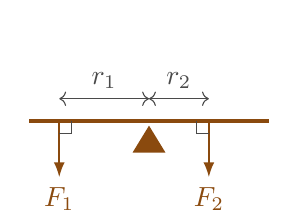
\begin{tikzpicture}[scale=0.95]
  \draw[koerper,line width=1.2pt] (-1.6,0)--(1.6,0);
  \fill[bern] (0,-0.06)--(-0.22,-0.42)--(0.22,-0.42)--cycle;
  \draw[vec] (-1.2,0)--(-1.2,-0.75) node[below,pos=1.0]{$F_1$};
  \draw[vec] (0.8,0)--(0.8,-0.75) node[below,pos=1.0]{$F_2$};
  \draw[grau,line width=0.4pt] (-1.04,0)--(-1.04,-0.16)--(-1.20,-0.16);
  \draw[grau,line width=0.4pt] (0.64,0)--(0.64,-0.16)--(0.80,-0.16);
  \draw[<->,grau,line width=0.4pt] (-1.2,0.3)--(0,0.3) node[midway,above]{$r_1$};
  \draw[<->,grau,line width=0.4pt] (0,0.3)--(0.8,0.3) node[midway,above]{$r_2$};
\end{tikzpicture}
\fcap{Hebel im Gleichgewicht: \(F_1r_1=F_2r_2\)}
\par}
\end{minipage}
\par\vspace{1.6mm}

\begin{minipage}[t]{0.54\linewidth}\vspace{0pt}
\ftitelD{Gleichgewichtsbedingungen des starren Körpers}
\[ \sum_i \vec F_i = \vec 0 \quad\Longleftrightarrow\quad \sum F_x = 0,\ \ \sum F_y = 0 \]
\[ \mtxt{und}\qquad \sum_i M_i = 0 \]
\hinweis{Rezept: Freikörperbild zeichnen, Drehpunkt geschickt wählen (dort verschwindet eine unbekannte Kraft im Momentensatz), dann auflösen.}
\end{minipage}\hfill
\begin{minipage}[t]{0.44\linewidth}\vspace{0pt}
{\centering\tikzfont
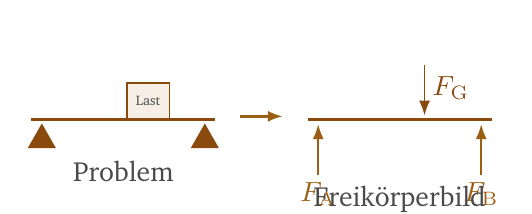
\begin{tikzpicture}[scale=0.90]
  % --- Problemskizze ---
  \draw[koerper,line width=1.1pt] (0,0)--(2.6,0);
  \fill[bern] (0.15,-0.05)--(-0.05,-0.40)--(0.35,-0.40)--cycle;
  \fill[bern] (2.45,-0.05)--(2.25,-0.40)--(2.65,-0.40)--cycle;
  \draw[koerper,fill=bernl] (1.35,0.02) rectangle (1.95,0.52);
  \node[grau] at (1.65,0.27) {\tiny Last};
  \node[grau] at (1.30,-0.72) {Problem};
  % --- Pfeil ---
  \draw[vecg,line width=0.9pt] (2.95,0.05)--(3.55,0.05);
  % --- Freikoerperbild ---
  \begin{scope}[xshift=3.9cm]
    \draw[koerper,line width=1.1pt] (0,0)--(2.6,0);
    \draw[vec] (1.65,0.78)--(1.65,0.06);
    \node[bern,right,inner sep=2pt] at (1.68,0.45) {$F_{\mathrm{G}}$};
    \draw[vecg] (0.15,-0.78)--(0.15,-0.06);
    \node[bernm,below,inner sep=2pt] at (0.15,-0.80) {$F_{\mathrm{A}}$};
    \draw[vecg] (2.45,-0.78)--(2.45,-0.06);
    \node[bernm,below,inner sep=2pt] at (2.45,-0.80) {$F_{\mathrm{B}}$};
    \node[grau] at (1.30,-1.12) {Freikörperbild};
  \end{scope}
\end{tikzpicture}
\fcap{Auflager durch ihre Kräfte ersetzen -- danach nur noch Vektoren}
\par}
\end{minipage}
\par\vspace{1.6mm}

\begin{minipage}[t]{0.54\linewidth}\vspace{0pt}
\ftitel{Balken auf zwei Stützen}
\hinweisD{Ansatz -- beide Gleichgewichtsbedingungen in Grundform:}
\[ \begin{array}{@{}l@{\ \ }l@{}}
   \mtxt{Momentengleichung um } A: & F_{\mathrm{G}}\cdot x = F_{\mathrm{B}}\cdot l\\[0.7ex]
   \mtxt{Kräftegleichung:} & F_{\mathrm{A}} + F_{\mathrm{B}} = F_{\mathrm{G}}
   \end{array} \]
\hinweis{Die Momentengleichung liefert \(F_{\mathrm{B}}\), die Kräftegleichung anschliessend \(F_{\mathrm{A}}\).
Mehrere Lasten: Momente einzeln aufsummieren.}
\end{minipage}\hfill
\begin{minipage}[t]{0.44\linewidth}\vspace{0pt}
\begin{leg}
F_{\mathrm{A}},F_{\mathrm{B}} & Auflagerkräfte in \(A\) und \(B\) & N\\
F_{\mathrm{G}} & Last & N\\
x & Abstand der Last vom Auflager \(A\) & m\\
l & Stützweite & m
\end{leg}
{\centering\tikzfont
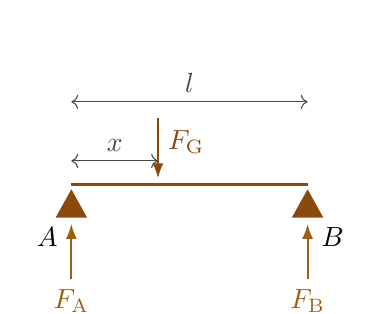
\begin{tikzpicture}[scale=1.0]
  \draw[koerper,line width=1.2pt] (0,0)--(3.0,0);
  \fill[bern] (0,-0.06)--(-0.2,-0.42)--(0.2,-0.42)--cycle;
  \fill[bern] (3.0,-0.06)--(2.8,-0.42)--(3.2,-0.42)--cycle;
  \node[below left] at (-0.05,-0.42) {$A$}; \node[below right] at (3.05,-0.42) {$B$};
  \draw[vec] (1.1,0.85)--(1.1,0.08) node[right,pos=0.4]{$F_{\mathrm{G}}$};
  \draw[vecg] (0,-1.2)--(0,-0.5) node[below,pos=0.0]{$F_{\mathrm{A}}$};
  \draw[vecg] (3.0,-1.2)--(3.0,-0.5) node[below,pos=0.0]{$F_{\mathrm{B}}$};
  \draw[<->,grau,line width=0.4pt] (0,0.3)--(1.1,0.3) node[midway,above]{$x$};
  \draw[<->,grau,line width=0.4pt] (0,1.05)--(3.0,1.05) node[midway,above]{$l$};
\end{tikzpicture}
\fcap{Momentensatz um \(A\): \(F_{\mathrm{B}}\,l = F_{\mathrm{G}}\,x\)}
\par}
\end{minipage}
\par\vspace{1.6mm}

\begin{minipage}[t]{0.54\linewidth}\vspace{0pt}
\ftitel{Seilkräfte an einer Aufhängung}
\hinweisD{\textbf{1. Ansatz} -- Gleichgewicht am Knoten, Kräfte in Komponenten zerlegt:}
\[ \begin{array}{@{}l@{\quad}l@{}}
   \sum F_x = 0: & F_{\mathrm{S2}}\cos\beta = F_{\mathrm{S1}}\cos\alpha\\[0.7ex]
   \sum F_y = 0: & F_{\mathrm{S1}}\sin\alpha + F_{\mathrm{S2}}\sin\beta = F_{\mathrm{G}}
   \end{array} \]
\hinweisD{\textbf{2. Auflösen} -- \(F_{\mathrm{S2}}\) aus der ersten Gleichung in die zweite einsetzen:}
\[ F_{\mathrm{S1}}\sin\alpha + F_{\mathrm{S1}}\frac{\cos\alpha}{\cos\beta}\sin\beta = F_{\mathrm{G}} \]
\[ F_{\mathrm{S1}}\cdot\frac{\sin\alpha\cos\beta+\cos\alpha\sin\beta}{\cos\beta} = F_{\mathrm{G}}
   \anm{Additionstheorem} \]
\hinweisD{\textbf{3. Ergebnis} -- mit \(\sin\alpha\cos\beta+\cos\alpha\sin\beta = \sin(\alpha+\beta)\):}
\[ F_{\mathrm{S1}} = F_{\mathrm{G}}\cdot\frac{\cos\beta}{\sin(\alpha+\beta)}\qquad
   F_{\mathrm{S2}} = F_{\mathrm{G}}\cdot\frac{\cos\alpha}{\sin(\alpha+\beta)} \]
\hinweis{Das flachere Seil trägt mehr: bei \(\alpha\to 0\) wächst \(F_{\mathrm{S1}}\) stark an.
Hängt die Last mittig, ist \(\alpha=\beta\) und beide Seilkräfte sind gleich.}
\end{minipage}\hfill
\begin{minipage}[t]{0.44\linewidth}\vspace{0pt}
\begin{leg}
F_{\mathrm{S1}},F_{\mathrm{S2}} & Seilkräfte & N\\
\alpha,\beta & Winkel der Seile zur Waagrechten & \(^\circ\)\\
F_{\mathrm{G}} & Last am Knoten & N
\end{leg}
{\centering\tikzfont
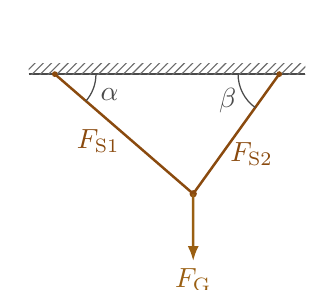
\begin{tikzpicture}[scale=0.95]
  \draw[grau,line width=0.7pt] (-1.85,1.60)--(1.85,1.60);
  \fill[pattern=north east lines,pattern color=hgrau] (-1.85,1.60) rectangle (1.85,1.74);
  \coordinate (A) at (-1.50,1.60);
  \coordinate (B) at (1.50,1.60);
  \coordinate (K) at (0.35,0.00);
  \draw[bern,line width=0.9pt] (A)--(K);
  \draw[bern,line width=0.9pt] (B)--(K);
  \fill[bern] (A) circle (1.1pt); \fill[bern] (B) circle (1.1pt); \fill[bern] (K) circle (1.4pt);
  \draw[grau,line width=0.45pt] ($(A)+(0:0.55)$) arc (0:-40.9:0.55);
  \node[grau] at (-0.77,1.33) {$\alpha$};
  \draw[grau,line width=0.45pt] ($(B)+(180:0.55)$) arc (180:234.3:0.55);
  \node[grau] at (0.81,1.24) {$\beta$};
  \node[bern] at (-0.92,0.70) {$F_{\mathrm{S1}}$};
  \node[bern] at (1.13,0.53) {$F_{\mathrm{S2}}$};
  \draw[vecg,line width=0.9pt] (K)--(0.35,-0.90);
  \node[bernm,below,inner sep=2pt] at (0.35,-0.92) {$F_{\mathrm{G}}$};
\end{tikzpicture}
\fcap{Last hängt aussermittig -- deshalb \(\alpha\neq\beta\); beide Winkel gegen die Waagrechte}
\par}
\end{minipage}
\par\vspace{1.6mm}


\TG[https://go4exercises.github.io/TALS-Physik/themen/p4-5-hydrostatik.html]{4.5}{Hydrostatik}\begin{minipage}[t]{0.54\linewidth}\vspace{0pt}
\ftitelD{Druck und Dichte}
\[ p = \frac{F}{A} \qquad\qquad \rho = \frac{m}{V}\quad\Longleftrightarrow\quad m = \rho\cdot V \]
\hinweis{\(1\;\ME{bar}=10^5\;\ME{Pa}=100\;\ME{kPa}\); Luftdruck auf Meereshöhe \(\approx 1013\;\ME{hPa}\).}
\end{minipage}\hfill
\begin{minipage}[t]{0.44\linewidth}\vspace{0pt}
\begin{leg}
p & Druck & Pa \(=\ME{N/m^2}\)\\
F & Kraft senkrecht auf die Fläche & N\\
A & Fläche & m\(^2\)\\
\rho & Dichte & kg/m\(^3\)\\
V & Volumen & m\(^3\)
\end{leg}
\end{minipage}
\par\vspace{1.6mm}

\begin{minipage}[t]{0.54\linewidth}\vspace{0pt}
\ftitelD{Schweredruck in einer Flüssigkeit}
\[ p_{\mathrm{S}} = \rho\cdot g\cdot h \qquad\qquad p_{\text{ges}} = p_0 + \rho\,g\,h \]
\gilt{ruhende, homogene und praktisch inkompressible Flüssigkeit, konstantes \(g\).}
\hinweis{Nur die \emph{Tiefe} zählt, nicht die Gefässform (hydrostatisches Paradoxon). In Wasser: rund \(1\;\ME{bar}\) pro \(10\;\ME{m}\).}
\end{minipage}\hfill
\begin{minipage}[t]{0.44\linewidth}\vspace{0pt}
\begin{leg}
p_{\mathrm{S}} & Schweredruck & Pa\\
h & Tiefe unter der Oberfläche & m\\
p_0 & Druck an der Oberfläche & Pa
\end{leg}
{\centering\tikzfont
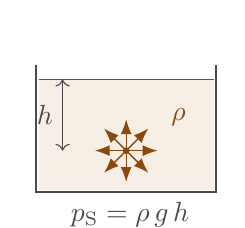
\begin{tikzpicture}[scale=0.95]
  \draw[grau,line width=0.7pt] (0,1.7)--(0,0)--(2.4,0)--(2.4,1.7);
  \fill[bernl] (0.03,0.03) rectangle (2.37,1.5);
  \draw[bern,line width=0.6pt] (0.03,1.5)--(2.37,1.5);
  \coordinate (Q) at (1.2,0.55);
  \fill[bern] (Q) circle (1.3pt);
  \foreach \a in {0,45,...,315}{\draw[vec,line width=0.5pt] (Q)--++(\a:0.42);}
  \draw[<->,grau,line width=0.4pt] (0.35,1.5)--(0.35,0.55) node[midway,left]{$h$};
  \node[bern] at (1.9,1.0) {$\rho$};
  \node[grau] at (1.25,-0.3) {$p_{\mathrm{S}}=\rho\,g\,h$};
\end{tikzpicture}
\fcap{Druck wirkt in alle Richtungen gleich}
\par}
\end{minipage}
\par\vspace{1.6mm}

\begin{minipage}[t]{0.54\linewidth}\vspace{0pt}
\ftitelD{Kommunizierende Röhren}
\[ \rho_1\cdot h_1 = \rho_2\cdot h_2 \]
\hinweis{\textbf{Eine} Flüssigkeit: in allen verbundenen Gefässen steht sie \emph{gleich hoch} --
unabhängig von Form und Querschnitt.}
\hinweis{\textbf{Zwei} nicht mischbare Flüssigkeiten: gleicher Druck in gleicher Höhe (Trennfläche).
Die \emph{leichtere} steht höher; die Höhen verhalten sich umgekehrt wie die Dichten:
\(h_1/h_2 = \rho_2/\rho_1\).}
\gilt{freie Oberflächen unter \emph{gleichem} Aussendruck; \(h_1\) und \(h_2\) ab derselben Trennfläche messen.}
\end{minipage}\hfill
\begin{minipage}[t]{0.44\linewidth}\vspace{0pt}
\begin{leg}
\rho_1,\rho_2 & Dichten der Flüssigkeiten & kg/m\(^3\)\\
h_1,h_2 & Höhen über der Trennfläche & m
\end{leg}
{\centering\tikzfont
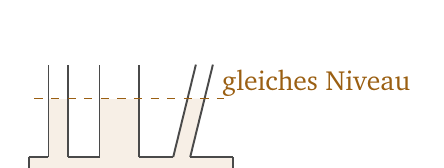
\begin{tikzpicture}[scale=0.72]
  \fill[bernl] (0.02,0.02) rectangle (3.58,0.32);
  \fill[bernl] (0.35,0.32) rectangle (0.70,1.35);
  \fill[bernl] (1.25,0.32) rectangle (1.95,1.35);
  \fill[bernl] (2.55,0.32)--(2.85,0.32)--(3.103,1.35)--(2.803,1.35)--cycle;
  \draw[grau,line width=0.7pt] (0,0.32)--(0,0)--(3.6,0)--(3.6,0.32);
  \draw[grau,line width=0.7pt] (0,0.32)--(0.35,0.32); \draw[grau,line width=0.7pt] (0.70,0.32)--(1.25,0.32);
  \draw[grau,line width=0.7pt] (1.95,0.32)--(2.55,0.32); \draw[grau,line width=0.7pt] (2.85,0.32)--(3.6,0.32);
  \draw[grau,line width=0.7pt] (0.35,0.32)--(0.35,1.95); \draw[grau,line width=0.7pt] (0.70,0.32)--(0.70,1.95);
  \draw[grau,line width=0.7pt] (1.25,0.32)--(1.25,1.95); \draw[grau,line width=0.7pt] (1.95,0.32)--(1.95,1.95);
  \draw[grau,line width=0.7pt] (2.55,0.32)--(2.95,1.95); \draw[grau,line width=0.7pt] (2.85,0.32)--(3.25,1.95);
  \draw[bernm,dashed,line width=0.5pt] (0.10,1.35)--(3.45,1.35);
  \node[bernm,right,inner sep=2pt] at (3.30,1.62) {gleiches Niveau};
\end{tikzpicture}
\fcap{eine Flüssigkeit: Form und Querschnitt spielen keine Rolle}
\vspace{2mm}

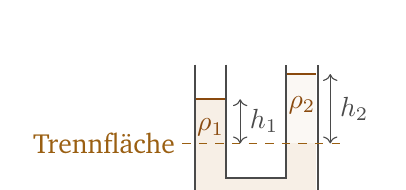
\begin{tikzpicture}[scale=0.80]
  \fill[bernl] (0.32,0.02) rectangle (2.23,0.30);
  \fill[bernl] (0.32,0.30) rectangle (0.78,1.55);
  \fill[bernl] (1.77,0.30) rectangle (2.23,0.85);
  \fill[bernl!45] (1.77,0.85) rectangle (2.23,1.95);
  \draw[grau,line width=0.7pt] (0.30,2.10)--(0.30,0)--(2.25,0)--(2.25,2.10);
  \draw[grau,line width=0.7pt] (0.80,2.10)--(0.80,0.30)--(1.75,0.30)--(1.75,2.10);
  \draw[bern,line width=0.6pt] (0.32,1.55)--(0.78,1.55);
  \draw[bern,line width=0.6pt] (1.77,1.95)--(2.23,1.95);
  \draw[bernm,dashed,line width=0.5pt] (0.10,0.85)--(2.60,0.85);
  \node[bernm,left,inner sep=2pt] at (0.08,0.85) {Trennfläche};
  \node[bern] at (0.55,1.10) {$\rho_1$};
  \node[bern] at (2.00,1.45) {$\rho_2$};
  \draw[<->,grau,line width=0.4pt] (1.02,0.85)--(1.02,1.55) node[midway,right]{$h_1$};
  \draw[<->,grau,line width=0.4pt] (2.45,0.85)--(2.45,1.95) node[midway,right]{$h_2$};
\end{tikzpicture}
\fcap{zwei Flüssigkeiten: die leichtere (\(\rho_2\)) steht höher}
\par}
\end{minipage}
\par\vspace{1.6mm}

\begin{minipage}[t]{0.54\linewidth}\vspace{0pt}
\ftitelD{Hydraulische Presse (Prinzip von Pascal)}
\[ \frac{F_1}{A_1} = \frac{F_2}{A_2} \qquad\Longrightarrow\qquad F_2 = F_1\cdot\frac{A_2}{A_1} \]
\[ s_1\cdot A_1 = s_2\cdot A_2 \qquad\Longrightarrow\qquad s_1 = s_2\cdot\frac{A_2}{A_1} \]
\hinweis{Kraftgewinn wird mit Weg bezahlt: die Arbeit \(W=F\,s\) bleibt gleich (Goldene Regel der Mechanik).}
\gilt{ideale, praktisch inkompressible Flüssigkeit; Reibung und Verluste vernachlässigt.}
\end{minipage}\hfill
\begin{minipage}[t]{0.44\linewidth}\vspace{0pt}
\begin{leg}
F_1,F_2 & Kolbenkräfte & N\\
A_1,A_2 & Kolbenflächen & m\(^2\)\\
s_1,s_2 & Kolbenwege & m
\end{leg}
{\centering\tikzfont
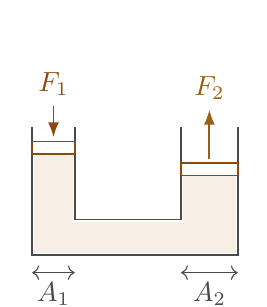
\begin{tikzpicture}[scale=0.9]
  \fill[bernl] (0.28,0.03) rectangle (3.12,0.47);
  \fill[bernl] (0.28,0.47) rectangle (0.82,1.42);
  \fill[bernl] (2.38,0.47) rectangle (3.12,1.12);
  \draw[grau,line width=0.7pt] (0.25,1.8)--(0.25,0)--(3.15,0)--(3.15,1.8);
  \draw[grau,line width=0.7pt] (0.85,1.8)--(0.85,0.5)--(2.35,0.5)--(2.35,1.8);
  \draw[koerper,fill=white] (0.25,1.42) rectangle (0.85,1.60);
  \draw[koerper,fill=white] (2.35,1.12) rectangle (3.15,1.30);
  \draw[vec] (0.55,2.10)--(0.55,1.66) node[above,pos=0.0]{$F_1$};
  \draw[vecg] (2.75,1.36)--(2.75,2.05) node[above,pos=1.0]{$F_2$};
  \draw[<->,grau,line width=0.4pt] (0.25,-0.25)--(0.85,-0.25) node[midway,below]{$A_1$};
  \draw[<->,grau,line width=0.4pt] (2.35,-0.25)--(3.15,-0.25) node[midway,below]{$A_2$};
\end{tikzpicture}
\fcap{kleine Fläche, kleine Kraft -- grosse Fläche, grosse Kraft}
\par}
\end{minipage}
\par\vspace{1.6mm}

\begin{minipage}[t]{0.54\linewidth}\vspace{0pt}
\ftitelD{Auftrieb (Prinzip von Archimedes)}
\[ F_{\mathrm{A}} = \rho_{\text{Fl}}\cdot V_{\mathrm{e}}\cdot g \]
\hinweis{\(F_{\mathrm{A}}\) entspricht der Gewichtskraft der verdrängten Flüssigkeit.}
\gilt{homogene Flüssigkeit und unverändertes eingetauchtes Volumen -- nur dann ist der Auftrieb unabhängig von der Tiefe.}
\end{minipage}\hfill
\begin{minipage}[t]{0.44\linewidth}\vspace{0pt}
\begin{leg}
F_{\mathrm{A}} & Auftriebskraft & N\\
\rho_{\text{Fl}} & Dichte der Flüssigkeit & kg/m\(^3\)\\
V_{\mathrm{e}} & verdrängtes (eingetauchtes) Volumen & m\(^3\)
\end{leg}
{\centering\tikzfont
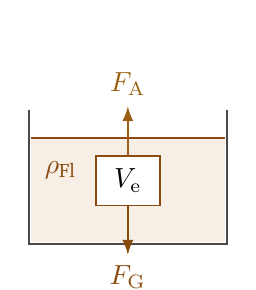
\begin{tikzpicture}[scale=0.9]
  \draw[grau,line width=0.7pt] (0,1.9)--(0,0)--(2.8,0)--(2.8,1.9);
  \fill[bernl] (0.03,0.03) rectangle (2.77,1.5);
  \draw[bern,line width=0.6pt] (0.03,1.5)--(2.77,1.5);
  \draw[koerper,fill=white] (0.95,0.55) rectangle (1.85,1.25);
  \node at (1.4,0.9) {$V_{\mathrm{e}}$};
  \draw[vecg] (1.4,1.25)--(1.4,1.95) node[above,pos=1.0]{$F_{\mathrm{A}}$};
  \draw[vec] (1.4,0.55)--(1.4,-0.15) node[below,pos=1.0]{$F_{\mathrm{G}}$};
  \node[bern] at (0.45,1.05) {$\rho_{\text{Fl}}$};
\end{tikzpicture}
\fcap{Auftrieb \(=\) Gewicht der verdrängten Flüssigkeit}
\par}
\end{minipage}
\par\vspace{1.6mm}

\begin{minipage}[t]{0.54\linewidth}\vspace{0pt}
\ftitelD{Schwimmen, Schweben, Sinken}
\[ \frac{V_{\mathrm{e}}}{V_{\mathrm{K}}} = \frac{\rho_{\mathrm{K}}}{\rho_{\text{Fl}}}\qquad
   \begin{cases}
     \rho_{\mathrm{K}} < \rho_{\text{Fl}} & \mtxt{schwimmt}\\
     \rho_{\mathrm{K}} = \rho_{\text{Fl}} & \mtxt{schwebt}\\
     \rho_{\mathrm{K}} > \rho_{\text{Fl}} & \mtxt{sinkt}
   \end{cases} \]
% ======================================================================
\end{minipage}\hfill
\begin{minipage}[t]{0.44\linewidth}\vspace{0pt}
\begin{leg}
V_{\mathrm{K}},\rho_{\mathrm{K}} & Volumen und Dichte des Körpers & m\(^3\), kg/m\(^3\)
\end{leg}
\end{minipage}
\par\vspace{1.6mm}

\addtocontents{toc}{\protect\columnbreak}
\LG{5}{Thermodynamik}\TG[https://go4exercises.github.io/TALS-Physik/themen/p5-1-temperatur.html]{5.1}{Temperatur}\begin{minipage}[t]{0.54\linewidth}\vspace{0pt}
\ftitelD{Temperaturskalen}
\[ T = \vartheta + 273.15 \qquad \vartheta = T - 273.15 \qquad \Delta T = \Delta\vartheta \]
\hinweis{Eine \emph{Differenz} von \(1\;\ME{K}\) ist gleich gross wie eine von \(1\;^\circ\)C -- in Differenz-Formeln
(\(Q=mc\Delta T\), \(\Delta l=\alpha l_0\Delta T\)) darf man deshalb beides einsetzen.}
\warn{Überall dort, wo \(T\) \emph{einzeln} oder als \emph{Quotient} auftritt, ist Kelvin zwingend:
in den Gasgesetzen sowie beim idealen COP und beim Carnot-Wirkungsgrad. Beim gewöhnlichen Wirkungsgrad
\(\eta=E_{\text{nutz}}/E_{\text{zu}}\) spielt die Temperatureinheit keine Rolle.}
\end{minipage}\hfill
\begin{minipage}[t]{0.44\linewidth}\vspace{0pt}
\begin{leg}
T & absolute Temperatur & K (Kelvin)\\
\vartheta & Celsius-Temperatur & \(^\circ\)C\\
\Delta T,\Delta\vartheta & Temperaturdifferenz & K
\end{leg}
{\centering\tikzfont
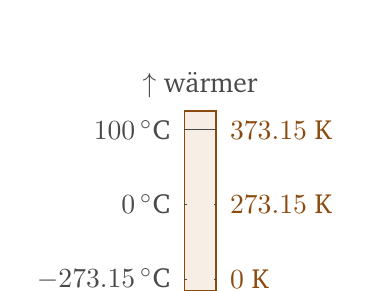
\begin{tikzpicture}[scale=0.95]
  \draw[koerper] (0,0) rectangle (0.42,2.4);
  \foreach \y/\c/\k in {0.15/-273.15/0, 1.15/0/273.15, 2.15/100/373.15}{
    \draw[grau,line width=0.5pt] (0,\y)--(0.42,\y);
    \node[left,grau] at (-0.06,\y) {$\c\,^\circ$C};
    \node[right,bern] at (0.48,\y) {$\k$ K};}
  \fill[bernl] (0.03,0.03) rectangle (0.39,1.15);
  \node[above,grau] at (0.21,2.45) {$\uparrow$ wärmer};
\end{tikzpicture}
\fcap{gleiche Schrittweite, verschobener Nullpunkt}
\par}
\end{minipage}
\par\vspace{1.6mm}

\ftitelD{Absoluter Nullpunkt}
\[ 0\;\ME{K} = -273.15\;^\circ\ME{C} \]
\hinweis{Tiefste mögliche Temperatur: die Teilchenbewegung ist minimal.
Im einfachen Teilchenmodell bzw.\ beim idealen Gas hängt die Temperatur mit der mittleren kinetischen Energie
der Teilchen zusammen.}

\needspace{4\baselineskip}\ftitelD{Fahrenheit (Praxis)}
\[ \vartheta_F = \tfrac{9}{5}\,\vartheta + 32 \qquad \vartheta = \tfrac{5}{9}\,(\vartheta_F - 32) \]

\TG[https://go4exercises.github.io/TALS-Physik/themen/p5-2-waerme.html]{5.2}{Wärme}\begin{minipage}[t]{0.54\linewidth}\vspace{0pt}
\ftitelD{Wärmemenge beim Erwärmen}
\[ Q = m\cdot c\cdot\Delta T \]
\hinweis{Wärme ist eine \emph{Prozessgrösse}: sie beschreibt die Energie\emph{übertragung}, nicht einen gespeicherten Vorrat.
Wasser hat mit \(c=4.19\;\ME{kJ/(kg\,K)}\) eine aussergewöhnlich hohe Wärmekapazität.}
\end{minipage}\hfill
\begin{minipage}[t]{0.44\linewidth}\vspace{0pt}
\begin{leg}
Q & übertragene Wärme & J\\
m & Masse & kg\\
c & spezifische Wärmekapazität & J/(kg\,K)\\
\Delta T & Temperaturänderung & K
\end{leg}
\end{minipage}
\par\vspace{1.6mm}

\begin{minipage}[t]{0.54\linewidth}\vspace{0pt}
\ftitelD{Wärmebilanz und Mischtemperatur}
\[ \sum_i Q_i = 0 \qquad\Longrightarrow\qquad
   \vartheta_m = \frac{m_1 c_1 \vartheta_1 + m_2 c_2 \vartheta_2}{m_1 c_1 + m_2 c_2} \]
\gilt{abgeschlossenes System ohne Wärmeverluste, kein Phasenwechsel, Wärmekapazität des Gefässes vernachlässigt.}
\hinweis{Abgegebene Wärme \(=\) aufgenommene Wärme, \(Q_{\text{ab}}<0\), \(Q_{\text{auf}}>0\).}
\end{minipage}\hfill
\begin{minipage}[t]{0.44\linewidth}\vspace{0pt}
\begin{leg}
\vartheta_m & Mischtemperatur & \(^\circ\)C\\
m_i,\vartheta_i & Masse und Anfangstemperatur & kg, \(^\circ\)C\\
c_i & spezifische Wärmekapazität & J/(kg\,K)
\end{leg}
\end{minipage}
\par\vspace{1.6mm}

\begin{minipage}[t]{0.54\linewidth}\vspace{0pt}
\ftitelD{Latente Wärme (Aggregatzustandswechsel)}
\[ Q = m\cdot L_{\text{f}} \quad\mtxt{(Schmelzen, Erstarren)} \]
\[ Q = m\cdot L_{\text{v}} \quad\mtxt{(Verdampfen, Kondensieren)} \]
\hinweis{Während des Phasenwechsels bleibt die Temperatur \emph{konstant} -- die Energie geht in die Umordnung der Teilchen.}
\end{minipage}\hfill
\begin{minipage}[t]{0.44\linewidth}\vspace{0pt}
\begin{leg}
L_{\text{f}} & spezifische Schmelzwärme & J/kg\\
L_{\text{v}} & spezifische Verdampfungswärme & J/kg
\end{leg}
{\centering\tikzfont
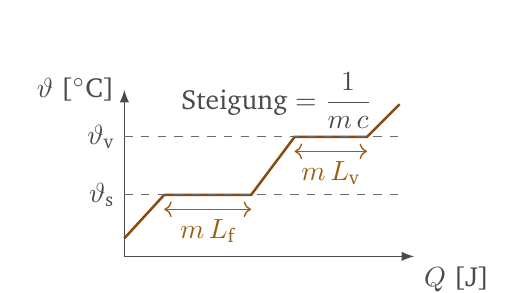
\begin{tikzpicture}[scale=0.92]
  \draw[ax] (0,0)--(4.0,0) node[below right]{$Q$ [J]};
  \draw[ax] (0,0)--(0,2.3) node[left]{$\vartheta$ [$^\circ$C]};
  \draw[kurve] (0,0.25)--(0.55,0.85)--(1.75,0.85)--(2.35,1.65)--(3.35,1.65)--(3.8,2.1);
  \draw[hilf] (0,0.85)--(3.8,0.85);
  \draw[hilf] (0,1.65)--(3.8,1.65);
  \node[left,grau] at (0,0.85) {$\vartheta_{\text{s}}$};
  \node[left,grau] at (0,1.65) {$\vartheta_{\text{v}}$};
  \draw[<->,bernm,line width=0.5pt] (0.55,0.65)--(1.75,0.65) node[midway,below]{$m\,L_{\text{f}}$};
  \draw[<->,bernm,line width=0.5pt] (2.35,1.45)--(3.35,1.45) node[midway,below]{$m\,L_{\text{v}}$};
  \node[grau] at (2.1,2.15) {Steigung $=\dfrac{1}{m\,c}$};
\end{tikzpicture}
\fcap{Heizkurve: schräg \(=\) erwärmen, waagrecht \(=\) Phasenwechsel}
\par}
\end{minipage}
\par\vspace{1.6mm}

\begin{minipage}[t]{0.54\linewidth}\vspace{0pt}
\ftitelD{Leistung und Wirkungsgrad}
\[ P = \frac{E}{t}\qquad \eta = \frac{E_{\text{nutz}}}{E_{\text{zu}}}\le 1 \]
\end{minipage}\hfill
\begin{minipage}[t]{0.44\linewidth}\vspace{0pt}
\begin{leg}
P & Leistung & W\\
\eta & Wirkungsgrad & --
\end{leg}
\end{minipage}
\par\vspace{1.6mm}

\begin{minipage}[t]{0.54\linewidth}\vspace{0pt}
\ftitelD{Wärmepumpe}
\[ \mtxt{COP} = \frac{Q_{\text{warm}}}{E_{\text{el}}}\qquad
   \mtxt{COP}_{\text{Carnot}} = \frac{T_{\text{warm}}}{T_{\text{warm}}-T_{\text{kalt}}} \]
\hinweis{\(\text{COP}>1\), weil Umgebungswärme mitgenutzt wird.}
\gilt{\(\text{COP}_{\text{Carnot}}\) ist der ideale, reversible Grenzfall -- reale Anlagen bleiben darunter.
\(T\) zwingend in Kelvin.}
\end{minipage}\hfill
\begin{minipage}[t]{0.44\linewidth}\vspace{0pt}
\begin{leg}
\text{COP} & Leistungszahl & --\\
\text{COP}_{\text{Carnot}} & idealer reversibler Grenzwert & --\\
T & Temperaturen in Kelvin & K
\end{leg}
\end{minipage}
\par\vspace{1.6mm}

\begin{minipage}[t]{0.54\linewidth}\vspace{0pt}
\ftitelD{Heizwert und Brennwert}
\[ E_{\text{chem}} = m\cdot H \qquad E_{\text{nutz}} = \eta\cdot m\cdot H \]
\[ \mtxt{bei Gasen volumenbezogen:}\qquad E_{\text{chem}} = V\cdot H \]
\gilt{vollständige Verbrennung; \(H\) ist ein Stoffkennwert.}
\hinweis{Der \emph{Heizwert} \(H_{\mathrm{i}}\) zählt die Verbrennungswärme ohne die Kondensationswärme des Wasserdampfs,
der \emph{Brennwert} \(H_{\mathrm{s}}\) mit -- deshalb ist \(H_{\mathrm{s}}>H_{\mathrm{i}}\). Brennwertheizungen nutzen genau diese Differenz.
Bei Gasen wird \(H\) meist auf das \emph{Normvolumen} bezogen -- dann in \(\ME{J/m^3}\) statt \(\ME{J/kg}\).}
\end{minipage}\hfill
\begin{minipage}[t]{0.44\linewidth}\vspace{0pt}
\begin{leg}
E_{\text{chem}} & freigesetzte chemische Energie & J\\
E_{\text{nutz}} & nutzbare Energie & J\\
m & Brennstoffmasse (fest, flüssig) & kg\\
V & Brennstoffvolumen (Gase) & m\(^3\)\\
H & Heizwert bzw.\ Brennwert & J/kg bzw.\ J/m\(^3\)\\
\eta & Wirkungsgrad der Anlage & --
\end{leg}
\end{minipage}
\par\vspace{1.6mm}

\ftitel{Wärmetransport -- drei Mechanismen}
\hinweis{\textbf{Wärmeleitung}: Energie wandert durch Stösse im Material, ohne Materietransport (Metalle gut, Luft schlecht). \quad
\textbf{Konvektion}: Transport durch strömende Flüssigkeiten oder Gase. \quad
\textbf{Wärmestrahlung}: elektromagnetische Wellen, funktioniert auch im Vakuum (Sonne).}
\par\vspace{1.6mm}

\begin{minipage}[t]{0.50\linewidth}\vspace{0pt}
\ftitel{Energiebilanz der Erde und Treibhauseffekt}
\hinweis{Die Sonne strahlt überwiegend \textbf{kurzwellig}: UV, sichtbares Licht und nahes Infrarot.
Ein Teil wird von Wolken, Eis und Boden
\emph{reflektiert}, der Rest \emph{absorbiert} und erwärmt die Oberfläche.}
\hinweis{Die erwärmte Erde strahlt \textbf{langwellig} (Infrarot) ab. Treibhausgase (CO\(_2\), CH\(_4\), H\(_2\)O)
lassen kurzwellige Strahlung weitgehend durch, absorbieren aber langwellige und strahlen einen Teil zurück
(\emph{Gegenstrahlung}).}
\merk{Im Gleichgewicht gilt: aufgenommene Leistung \(=\) abgegebene Leistung. Mehr Treibhausgase \(\Rightarrow\)
das Gleichgewicht stellt sich bei \emph{höherer} Oberflächentemperatur ein.}
\end{minipage}\hfill
\begin{minipage}[t]{0.48\linewidth}\vspace{0pt}
{\centering\tikzfont
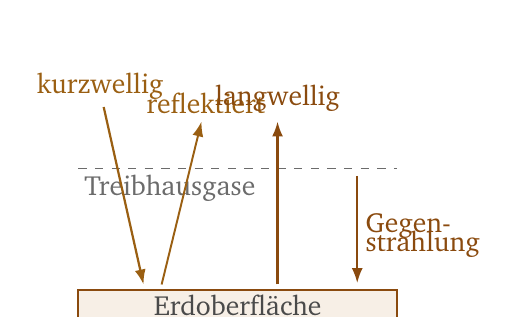
\begin{tikzpicture}[scale=0.92]
  \fill[bernl] (0,0) rectangle (4.4,0.42);
  \draw[koerper,line width=0.7pt] (0,0) rectangle (4.4,0.42);
  \node[grau] at (2.2,0.21) {Erdoberfläche};
  \draw[hgrau,dashed,line width=0.5pt] (0,2.10)--(4.4,2.10);
  \node[hgrau,below right,inner sep=1.5pt] at (0.02,2.08) {Treibhausgase};
  \draw[vecg,line width=0.8pt] (0.35,2.95)--(0.90,0.50);
  \node[bernm,above] at (0.30,2.92) {kurzwellig};
  \draw[vecg] (1.15,0.50)--(1.70,2.75);
  \node[bernm,above] at (1.76,2.72) {reflektiert};
  \draw[vec,line width=0.8pt] (2.75,0.50)--(2.75,2.75);
  \node[bern,above] at (2.75,2.75) {langwellig};
  \draw[vec] (3.85,2.00)--(3.85,0.52);
  \node[bern,right,inner sep=1.5pt] at (3.90,1.30) {Gegen-};
  \node[bern,right,inner sep=1.5pt] at (3.90,1.05) {strahlung};
\end{tikzpicture}
\fcap{kurzwellig hinein, langwellig hinaus -- Treibhausgase bremsen den Ausgang}
\par}
\end{minipage}

\TG[https://go4exercises.github.io/TALS-Physik/themen/p5-3-waermeausdehnung.html]{5.3}{Wärmeausdehnung}\begin{minipage}[t]{0.54\linewidth}\vspace{0pt}
\ftitelD{Längenausdehnung}
\[ \Delta l = \alpha\cdot l_0\cdot\Delta T \qquad l = l_0 + \Delta l = l_0\,(1+\alpha\,\Delta T) \]
\hinweis{\(\alpha\) liegt bei Metallen in der Grössenordnung \(10^{-5}\;\ME{K^{-1}}\). Dehnungsfugen bei Brücken und Schienen.}
\end{minipage}\hfill
\begin{minipage}[t]{0.44\linewidth}\vspace{0pt}
\begin{leg}
\Delta l & Längenänderung & m\\
l_0 & Ausgangslänge & m\\
\alpha & Längenausdehnungskoeffizient & 1/K\\
\Delta T & Temperaturänderung & K
\end{leg}
{\centering\tikzfont
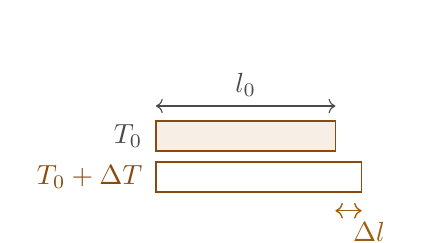
\begin{tikzpicture}[scale=0.95]
  \draw[koerper] (0,0.55) rectangle (2.4,0.95);
  \draw[koerper,fill=white] (0,0) rectangle (2.75,0.4);
  \draw[<->,grau,line width=0.4pt] (0,1.15)--(2.4,1.15) node[midway,above]{$l_0$};
  \draw[<->,bernm,line width=0.5pt] (2.4,-0.25)--(2.75,-0.25);
  \node[below,bernm] at (2.85,-0.28) {$\Delta l$};
  \node[left,grau] at (-0.05,0.75) {$T_0$};
  \node[left,bern] at (-0.05,0.2) {$T_0+\Delta T$};
\end{tikzpicture}
\fcap{Ausdehnung ist proportional zu \(l_0\) und \(\Delta T\)}
\par}
\end{minipage}
\par\vspace{1.6mm}

\begin{minipage}[t]{0.54\linewidth}\vspace{0pt}
\ftitelD{Volumenausdehnung}
\[ \Delta V = \gamma\cdot V_0\cdot\Delta T \]
\[ \mtxt{isotrope Festkörper:}\qquad \gamma \approx 3\,\alpha \]
\hinweis{Flüssigkeiten dehnen sich deutlich stärker aus als Festkörper, Gase noch stärker.}
\end{minipage}\hfill
\begin{minipage}[t]{0.44\linewidth}\vspace{0pt}
\begin{leg}
\Delta V & Volumenänderung & m\(^3\)\\
\gamma & Volumenausdehnungskoeffizient & 1/K
\end{leg}
\end{minipage}
\par\vspace{1.6mm}

\ftitelD{Dichte in Abhängigkeit der Temperatur}
\[ \rho = \frac{\rho_0}{1+\gamma\cdot\Delta T} \]
\hinweis{Erwärmen \(\to\) grösseres Volumen bei gleicher Masse \(\to\) kleinere Dichte (Auftrieb, Konvektion, Heissluftballon).
\textbf{Wasseranomalie}: grösste Dichte bei \(4\,^\circ\)C -- Seen frieren von oben zu.}

\begin{minipage}[t]{0.54\linewidth}\vspace{0pt}
\ftitelD{Allgemeines Gasgesetz}
\[ \frac{p\cdot V}{T} = \mtxt{konstant} \qquad\Longleftrightarrow\qquad
   \frac{p_1 V_1}{T_1} = \frac{p_2 V_2}{T_2} \]
\gilt{konstante Stoffmenge eines idealen bzw.\ näherungsweise idealen Gases; \(T\) in Kelvin, \(p\) als absoluter Druck.}
\zwiD{\textbf{Drei Sonderfälle} -- je eine Grösse wird festgehalten:}
\[ \begin{array}{@{}l@{\quad}l@{\quad}l@{}}
   T = \mtxt{konst.} & p\cdot V = \mtxt{konst.} & \anm{Boyle-Mariotte}\\[0.8ex]
   V = \mtxt{konst.} & \dfrac{p}{T} = \mtxt{konst.} & \anm{Amontons}\\[1.4ex]
   p = \mtxt{konst.} & \dfrac{V}{T} = \mtxt{konst.} & \anm{Gay-Lussac}
   \end{array} \]
\hinweis{\textbf{Alltag.}\ \ \emph{Boyle-Mariotte}: Velopumpe zuhalten und den Kolben \emph{langsam}
eindrücken -- das Volumen wird kleiner, der Druck steigt. Nur bei langsamem Vorgang und ausreichendem
Wärmeaustausch ist das näherungsweise isotherm; schnelles Eindrücken erwärmt die Luft.\ \
\emph{Amontons}: Autoreifen nach schneller Fahrt oder Spraydose in der Sonne -- das Volumen ist fest, mit der Temperatur
steigt der Druck.\ \
\emph{Gay-Lussac}: Luftballon im Kühlschrank schrumpft, über der Heizung dehnt er sich -- der Aussendruck bleibt gleich.}
\warn{Die beiden Geraden gehen nur durch den Ursprung, wenn \(T\) in \textbf{Kelvin} eingesetzt wird.
Extrapoliert man das ideale Gasmodell, so geht bei konstantem Volumen der \emph{Druck} und bei konstantem
Druck das \emph{Volumen} für \(T\to 0\;\ME{K}\) gegen null. Reale Gase kondensieren jedoch vorher, und
\(0\;\ME{K}\) wird nicht erreicht. Historisch trug genau diese Extrapolation zur Bestimmung des absoluten
Nullpunkts bei.}
\end{minipage}\hfill
\begin{minipage}[t]{0.44\linewidth}\vspace{0pt}
\begin{leg}
p & absoluter Druck & Pa\\
V & Volumen & m\(^3\)\\
T & absolute Temperatur & K
\end{leg}
{\centering\tikzfont
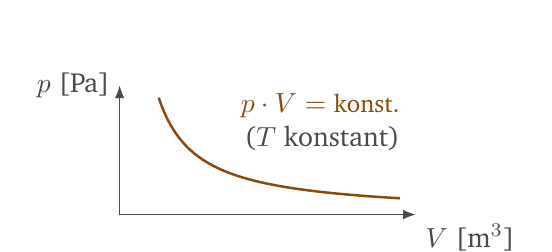
\begin{tikzpicture}[scale=0.80]
  \draw[ax] (0,0)--(4.70,0) node[below right]{$V$ [m$^3$]};
  \draw[ax] (0,0)--(0,2.05) node[left]{$p$ [Pa]};
  \draw[kurve,domain=0.62:4.45,samples=80,variable=\x] plot ({\x},{1.15/\x});
  \node[bern,anchor=east] at (4.60,1.72) {$p\cdot V=\mtxt{konst.}$};
  \node[grau,anchor=east] at (4.60,1.22) {($T$ konstant)};
\end{tikzpicture}
\fcap{Isotherme -- Boyle-Mariotte: Velopumpe}
\vspace{2mm}

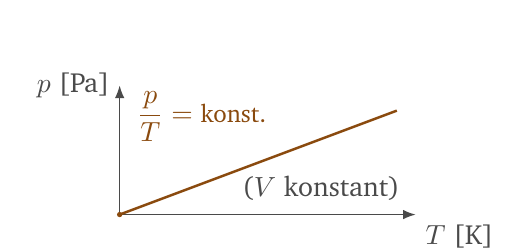
\begin{tikzpicture}[scale=0.80]
  \draw[ax] (0,0)--(4.70,0) node[below right]{$T$ [K]};
  \draw[ax] (0,0)--(0,2.05) node[left]{$p$ [Pa]};
  \draw[kurve] (0,0)--(4.40,1.65);
  \node[bern,anchor=north west] at (0.12,2.10) {$\dfrac{p}{T}=\mtxt{konst.}$};
  \node[grau,anchor=east] at (4.60,0.42) {($V$ konstant)};
  \fill[bern] (0,0) circle (1.2pt);
\end{tikzpicture}
\fcap{Isochore -- Amontons: Reifen, Spraydose}
\vspace{2mm}

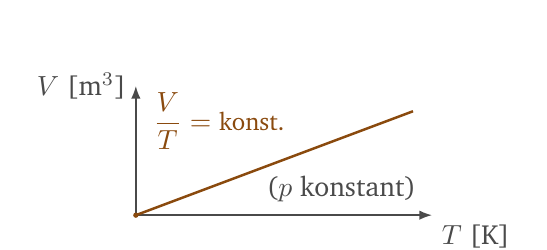
\begin{tikzpicture}[scale=0.80]
  \draw[ax] (0,0)--(4.70,0) node[below right]{$T$ [K]};
  \draw[ax] (0,0)--(0,2.05) node[left]{$V$ [m$^3$]};
  \draw[kurve] (0,0)--(4.40,1.65);
  \node[bern,anchor=north west] at (0.12,2.10) {$\dfrac{V}{T}=\mtxt{konst.}$};
  \node[grau,anchor=east] at (4.60,0.42) {($p$ konstant)};
  \fill[bern] (0,0) circle (1.2pt);
\end{tikzpicture}
\fcap{Isobare -- Gay-Lussac: Ballon im Kühlschrank}
\par}
\end{minipage}
\par\vspace{1.6mm}

\LG{6}{Einführung in andere Bereiche der Physik}\TG[https://go4exercises.github.io/TALS-Physik/themen/p6-1-wellen.html]{6.1}{Wellen}\begin{minipage}[t]{0.54\linewidth}\vspace{0pt}
\ftitelD{Ein Seilpunkt über die Zeit -- die Schwingung}
\[ f = \frac{1}{T}\qquad T = \frac{1}{f}\qquad \omega = \frac{2\pi}{T} = 2\pi f \]
\[ y(t) = A\cdot\sin\!\left(2\pi\,\frac{t}{T} + \varphi\right) = A\cdot\sin(\omega\,t + \varphi) \]
\hinweis{Man beobachtet \emph{einen einzigen} Punkt des Seils und trägt seine Auslenkung über der Zeit auf.
Die \textbf{Phasenkonstante} \(\varphi\) legt fest, wo die Sinuskurve bei \(t=0\) startet:
\(\varphi = 0\) heisst Start in der Ruhelage nach oben, \(\varphi = \pi/2\) Start im oberen Umkehrpunkt.
Ein \emph{positives} \(\varphi\) verschiebt die Kurve nach \emph{links}, und zwar um
\(\Delta t = \dfrac{\varphi}{2\pi}\,T\) \ (\(\varphi\) in rad).}
\end{minipage}\hfill
\begin{minipage}[t]{0.44\linewidth}\vspace{0pt}
\begin{leg}
T & Schwingungsdauer (Periode) & s\\
f & Frequenz & Hz \(=1/\)s\\
\omega & Kreisfrequenz & rad/s\\
A & Amplitude (max.\ Auslenkung) & m\\
\varphi & Phasenkonstante & rad
\end{leg}
{\centering\tikzfont
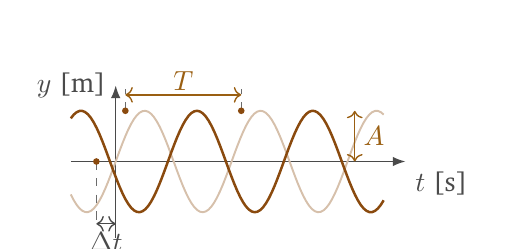
\begin{tikzpicture}[scale=0.92]
  \draw[ax] (-0.62,0)--(4.0,0) node[below right]{$t$ [s]};
  \draw[ax] (0,-1.05)--(0,1.05) node[left]{$y$ [m]};
  \draw[bern!35,line width=0.7pt,domain=-0.62:3.7,samples=110,variable=\x]
    plot ({\x},{0.7*sin(deg(2*pi*\x/1.6))});
  \draw[kurve,domain=-0.62:3.7,samples=110,variable=\x]
    plot ({\x},{0.7*sin(deg(2*pi*\x/1.6+60))});
  % Periode: von Wellenberg zu Wellenberg
  \draw[hilf] (0.1333,0.70)--(0.1333,1.00);
  \draw[hilf] (1.7333,0.70)--(1.7333,1.00);
  \fill[bern] (0.1333,0.70) circle (1.3pt);
  \fill[bern] (1.7333,0.70) circle (1.3pt);
  \draw[<->,bernm,line width=0.5pt] (0.1333,0.92)--(1.7333,0.92)
    node[midway,above,inner sep=1.5pt]{$T$};
  % Phasenverschiebung: Nulldurchgang der kraeftigen Kurve liegt um Delta t frueher
  \draw[hilf] (-0.2667,0)--(-0.2667,-0.86);
  \fill[bern] (-0.2667,0) circle (1.3pt);
  \draw[<->,grau,line width=0.5pt] (-0.2667,-0.86)--(0,-0.86);
  \node[grau,below,inner sep=2pt] at (-0.1333,-0.90) {$\Delta t$};
  \draw[<->,bernm,line width=0.5pt] (3.30,0)--(3.30,0.70);
  \node[bernm,right,inner sep=2pt] at (3.34,0.35) {$A$};
\end{tikzpicture}
\fcap{Ein Seilpunkt über die Zeit; \(T\) von Wellenberg zu Wellenberg.
Matt: \(\varphi=0\), kräftig: um \(\varphi\) verschoben -- die kräftige Kurve erreicht den Berg um \(\Delta t\) früher}
\par}
\end{minipage}
\par\vspace{1.6mm}

\begin{minipage}[t]{0.54\linewidth}\vspace{0pt}
\ftitelD{Das ganze Seil in einem Moment -- das Momentbild}
\[ c = \frac{\lambda}{T} = \lambda\cdot f \]
\[ y(s) = A\cdot\sin\!\left(2\pi\,\frac{s}{\lambda} + \delta\right) \]
\hinweis{Jetzt wird die Zeit festgehalten und das \emph{ganze} Seil auf einmal betrachtet -- wie ein Foto.
Ein \emph{positives} \(\delta\) verschiebt das Bild längs des Seils nach \emph{links}, und zwar um
\(\Delta s = \dfrac{\delta}{2\pi}\,\lambda\) \ (\(\delta\) in rad).}
\hinweis{Die Frequenz wird vom \emph{Sender} bestimmt und ändert sich beim Medienwechsel nicht; \(c\) hängt von Wellenart und
Medium ab, \(\lambda\) passt sich an. Schall in Luft (\(20\,^\circ\)C): \(c\approx 343\;\ME{m/s}\); Licht im Vakuum:
\(c = 3.00\cdot 10^{8}\;\ME{m/s}\).}
\end{minipage}\hfill
\begin{minipage}[t]{0.44\linewidth}\vspace{0pt}
\begin{leg}
c & Ausbreitungsgeschwindigkeit & m/s\\
\lambda & Wellenlänge & m\\
f & Frequenz & Hz\\
\delta & Phasenkonstante & rad
\end{leg}
{\centering\tikzfont
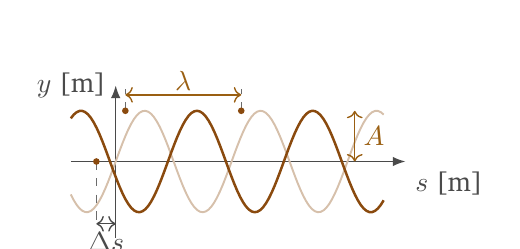
\begin{tikzpicture}[scale=0.92]
  \draw[ax] (-0.62,0)--(4.0,0) node[below right]{$s$ [m]};
  \draw[ax] (0,-1.05)--(0,1.05) node[left]{$y$ [m]};
  \draw[bern!35,line width=0.7pt,domain=-0.62:3.7,samples=110,variable=\x]
    plot ({\x},{0.7*sin(deg(2*pi*\x/1.6))});
  \draw[kurve,domain=-0.62:3.7,samples=110,variable=\x]
    plot ({\x},{0.7*sin(deg(2*pi*\x/1.6+60))});
  % Wellenlaenge: von Wellenberg zu Wellenberg
  \draw[hilf] (0.1333,0.70)--(0.1333,1.00);
  \draw[hilf] (1.7333,0.70)--(1.7333,1.00);
  \fill[bern] (0.1333,0.70) circle (1.3pt);
  \fill[bern] (1.7333,0.70) circle (1.3pt);
  \draw[<->,bernm,line width=0.5pt] (0.1333,0.92)--(1.7333,0.92)
    node[midway,above,inner sep=1.5pt]{$\lambda$};
  % Phasenverschiebung
  \draw[hilf] (-0.2667,0)--(-0.2667,-0.86);
  \fill[bern] (-0.2667,0) circle (1.3pt);
  \draw[<->,grau,line width=0.5pt] (-0.2667,-0.86)--(0,-0.86);
  \node[grau,below,inner sep=2pt] at (-0.1333,-0.90) {$\Delta s$};
  \draw[<->,bernm,line width=0.5pt] (3.30,0)--(3.30,0.70);
  \node[bernm,right,inner sep=2pt] at (3.34,0.35) {$A$};
\end{tikzpicture}
\fcap{Das ganze Seil in einem Moment; \(\lambda\) ist der Abstand zweier gleicher Phasen,
hier von Wellenberg zu Wellenberg}
\par}
\end{minipage}
\par\vspace{1.6mm}

\begin{minipage}[t]{0.54\linewidth}\vspace{0pt}
\ftitelD{Beides zusammen -- die laufende Welle}
\[ y(s,t) = A\cdot\sin\!\left(2\pi\left(\frac{t}{T}-\frac{s}{\lambda}\right)\right) \]
\hinweis{Diese Gleichung enthält beide Sichtweisen: Hält man den \emph{Ort} \(s\) fest, entsteht die Schwingung \(y(t)\);
hält man die \emph{Zeit} \(t\) fest, entsteht das Momentbild \(y(s)\). Die Phasenkonstanten \(\varphi\) und \(\delta\)
ergeben sich dabei aus dem gewählten Ort bzw.\ Zeitpunkt.}
\end{minipage}\hfill
\begin{minipage}[t]{0.44\linewidth}\vspace{0pt}
\begin{leg}
y & Auslenkung am Ort \(s\) zur Zeit \(t\) & m\\
s & Ort entlang der Ausbreitungsrichtung & m
\end{leg}
\end{minipage}
\par\vspace{1.6mm}

\ftitelD{Überlagerung (Superposition)}
\[ y = y_1 + y_2 \]
\hinweis{Auslenkungen addieren sich vorzeichenrichtig: gleichsinnig \(\to\) Verstärkung, gegensinnig \(\to\) Auslöschung.
Nach der Begegnung laufen beide Wellen unverändert weiter.}

\begin{minipage}[t]{0.54\linewidth}\vspace{0pt}
\ftitelD{Stehende Welle auf einer Saite (beidseitig fest)}
\[ L = n\cdot\frac{\lambda_n}{2}\qquad \lambda_n = \frac{2L}{n}\qquad
   f_n = \frac{c}{\lambda_n} = n\cdot\frac{c}{2L},\qquad n=1,2,3,\ldots \]
\gilt{beidseitig befestigte Saite -- an beiden Enden liegt ein Knoten.}
\hinweis{Die Obertöne sind ganzzahlige Vielfache des Grundtons \(f_1\). Kürzere Saite oder höhere Wellengeschwindigkeit
(mehr Spannung) \(\to\) höherer Ton. Für Pfeifen und Rohre gelten je nach offenen bzw.\ geschlossenen Enden
andere Randbedingungen.}
\end{minipage}\hfill
\begin{minipage}[t]{0.44\linewidth}\vspace{0pt}
\begin{leg}
L & Länge der beidseitig befestigten Saite & m\\
n & Ordnung (Grundton \(n=1\)) & --\\
\lambda_n & Wellenlänge der \(n\)-ten Mode & m\\
f_n & Eigenfrequenz (\(n\)-te Harmonische) & Hz
\end{leg}
{\centering\tikzfont
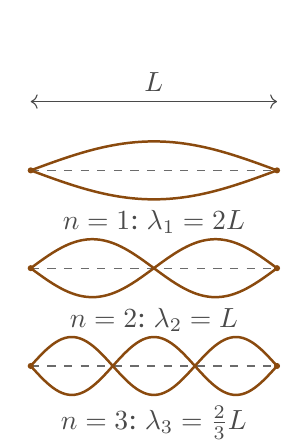
\begin{tikzpicture}[scale=0.92]
  \draw[<->,grau,line width=0.4pt] (0,0.95)--(3.4,0.95) node[midway,above]{$L$};
  \foreach \n/\y/\lab in {1/0/{$n=1$:\ $\lambda_1=2L$}, 2/-1.35/{$n=2$:\ $\lambda_2=L$}, 3/-2.7/{$n=3$:\ $\lambda_3=\tfrac{2}{3}L$}}{
    \begin{scope}[yshift=\y cm]
      \draw[hilf] (0,0)--(3.4,0);
      \draw[kurve,domain=0:3.4,samples=80,variable=\x] plot ({\x},{0.4*sin(deg(\n*pi*\x/3.4))});
      \draw[kurve,domain=0:3.4,samples=80,variable=\x] plot ({\x},{-0.4*sin(deg(\n*pi*\x/3.4))});
      \fill[bern] (0,0) circle (1.2pt); \fill[bern] (3.4,0) circle (1.2pt);
      \node[grau,below] at (1.7,-0.42) {\lab};
    \end{scope}}
\end{tikzpicture}
\fcap{Eigenschwingungen: an den Enden immer ein Knoten}
\par}
\end{minipage}
\par\vspace{1.6mm}

\ftitel{Wellenarten und Beispiele}
\hinweis{\textbf{Transversal} (Querwelle) -- Schwingung \(\perp\) Ausbreitungsrichtung:
Seilwelle, gespanntes \emph{Gummiband}, Querschwingung des Fahrbahnträgers einer \emph{Hängebrücke},
Licht und alle elektromagnetischen Wellen.}
\hinweis{\textbf{Longitudinal} (Längswelle) -- Schwingung \(\parallel\) Ausbreitungsrichtung:
Schall in Luft, Druckstoss in einer Flüssigkeit, Stauchwelle längs einer Schraubenfeder.}
\warn{\textbf{Wasserwellen} sind \emph{keiner} der beiden Arten rein zuzuordnen: die Wasserteilchen laufen auf
Kreis- bzw.\ Ellipsenbahnen -- eine Überlagerung aus Quer- und Längsbewegung.}
\merk{\textbf{Schwingung oder Welle?} \emph{Gummiband}, Federpendel und \emph{Stossdämpfer} sind zunächst
\textbf{Schwingungen}: ein einzelner Körper bewegt sich um seine Ruhelage. Zur \textbf{Welle} wird es erst, wenn sich
die Störung im Raum \emph{ausbreitet}. Der Stossdämpfer ist zudem eine \emph{gedämpfte} Schwingung -- die Energie wird
absichtlich in Wärme umgewandelt, die Amplitude nimmt ab.}
\hinweis{\textbf{Mechanische} Wellen brauchen ein Medium, \textbf{elektromagnetische} nicht.}

\begin{minipage}[t]{0.54\linewidth}\vspace{0pt}
\ftitel{Emission und Absorption}
\hinweis{Atome und Moleküle nehmen Energie nur in \emph{bestimmten Portionen} auf und geben sie so wieder ab.
Beim Übergang in einen \emph{tieferen} Energiezustand wird ein Photon ausgesandt. Seine Energie entspricht der
Energiedifferenz der beiden Zustände; sie bestimmt die Frequenz und bei sichtbarer Strahlung die Farbe:}
\[ E = h\cdot f \]
\hinweis{Umgekehrt wird ein Photon nur absorbiert, wenn seine Energie zu einem Übergang passt. Deshalb sind Stoffe
für manche Wellenlängen durchlässig und für andere nicht -- genau das erklärt die wellenlängenabhängige Absorption
in der Atmosphäre.}
\end{minipage}\hfill
\begin{minipage}[t]{0.44\linewidth}\vspace{0pt}
\begin{leg}
E & Energie des Photons & J\\
h & Planck-Konstante \(6.626\cdot10^{-34}\) & Js\\
f & Frequenz & Hz
\end{leg}
\end{minipage}
\par\vspace{1.6mm}

\ftitel{Elektromagnetisches Spektrum}
\hinweis{Radio \(\to\) Mikrowellen \(\to\) Infrarot \(\to\) \textbf{sichtbares Licht (\(380\)--\(780\;\ME{nm}\))} \(\to\) UV \(\to\) Röntgen \(\to\) Gamma.
Alle mit \(c = 3.00\cdot10^{8}\;\ME{m/s}\) im Vakuum: grosse Wellenlänge \(\Leftrightarrow\) kleine Frequenz.}

\TG[https://go4exercises.github.io/TALS-Physik/themen/p6-2-elektrizitaet.html]{6.2}{Elektrizität}\begin{minipage}[t]{0.54\linewidth}\vspace{0pt}
\ftitelD{Ladung und Stromstärke}
\[ I = \frac{Q}{t}\qquad Q = I\cdot t \qquad e = 1.602\cdot10^{-19}\;\ME{C} \]
\end{minipage}\hfill
\begin{minipage}[t]{0.44\linewidth}\vspace{0pt}
\begin{leg}
Q & elektrische Ladung & C \(=\ME{As}\)\\
I & Stromstärke & A\\
t & Zeit & s\\
e & Elementarladung & C
\end{leg}
\end{minipage}
\par\vspace{1.6mm}

\begin{minipage}[t]{0.54\linewidth}\vspace{0pt}
\ftitelD{Coulombkraft}
\[ F = k\cdot\frac{|Q_1\cdot Q_2|}{r^{\,2}}\qquad k = 8.99\cdot10^{9}\;\frac{\ME{N\,m^2}}{\ME{C^2}} \]
\hinweis{Die Formel liefert den \emph{Betrag}. Die Richtung folgt aus den Vorzeichen: gleichnamige Ladungen stossen sich ab,
ungleichnamige ziehen sich an. Doppelter Abstand \(\to\) ein Viertel der Kraft.}
\gilt{der angegebene Wert von \(k\) im Vakuum, in Luft näherungsweise. In anderen Medien ist die Kraft wegen
der Permittivität des Mediums kleiner.}
\end{minipage}\hfill
\begin{minipage}[t]{0.44\linewidth}\vspace{0pt}
\begin{leg}
F & \emph{Betrag} der Kraft zwischen zwei Ladungen & N\\
r & Abstand der Ladungen & m
\end{leg}
\end{minipage}
\par\vspace{1.6mm}

\begin{minipage}[t]{0.54\linewidth}\vspace{0pt}
\ftitelD{Spannung}
\[ U = \frac{W}{Q} \]
\end{minipage}\hfill
\begin{minipage}[t]{0.44\linewidth}\vspace{0pt}
\begin{leg}
U & elektrische Spannung & V \(=\ME{J/C}\)\\
W & Arbeit am Ladungstransport & J
\end{leg}
\end{minipage}
\par\vspace{1.6mm}

\begin{minipage}[t]{0.54\linewidth}\vspace{0pt}
\ftitelD{Ohmsches Gesetz}
\[ U = R\cdot I \qquad R = \frac{U}{I} \qquad I = \frac{U}{R} \]
\gilt{ohmscher Leiter bei konstanter Temperatur.}
\hinweis{\(R=U/I\) definiert den Widerstand immer; \emph{ohmsch} heisst, dass \(R\) dabei konstant bleibt.
Glühlampen, Dioden und Halbleiter verhalten sich nicht ohmsch.}
\merk{Das Gesetz gilt \textbf{doppelt}: für \emph{jeden einzelnen} Widerstand einer Schaltung
(\(U_1 = R_1 I_1\)) und für die \emph{ganze} Schaltung (\(U_{\text{ges}} = R_{\text{ges}} I_{\text{ges}}\)).
Entscheidend ist, dass \(U\), \(I\) und \(R\) zum \emph{selben} Bauteil gehören -- also die Spannung über genau dem
Widerstand, durch den der Strom \(I\) fliesst.}
\end{minipage}\hfill
\begin{minipage}[t]{0.44\linewidth}\vspace{0pt}
\begin{leg}
R & elektrischer Widerstand & \(\Omega = \ME{V/A}\)\\
U & Spannung über dem Widerstand & V\\
I & Strom durch den Widerstand & A
\end{leg}
{\centering\tikzfont
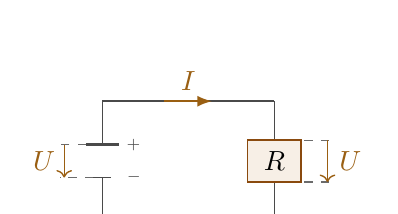
\begin{tikzpicture}[scale=0.95]
  \draw[grau,line width=0.6pt] (0.35,0)--(2.65,0);
  \draw[grau,line width=0.6pt] (2.65,0)--(2.65,0.52);
  \draw[grau,line width=0.6pt] (2.65,1.08)--(2.65,1.60);
  \draw[grau,line width=0.6pt] (2.65,1.60)--(0.35,1.60);
  \draw[grau,line width=0.6pt] (0.35,1.60)--(0.35,1.02);
  \draw[grau,line width=0.6pt] (0.35,0.58)--(0.35,0);
  \draw[grau,line width=1pt] (0.13,1.02)--(0.57,1.02);
  \draw[grau,line width=0.6pt] (0.23,0.58)--(0.47,0.58);
  \node[grau,right,inner sep=2pt] at (0.59,1.02) {\tiny$+$};
  \node[grau,right,inner sep=2pt] at (0.59,0.58) {\tiny$-$};
  \draw[hilf] (0.13,1.02)--(-0.22,1.02);
  \draw[hilf] (0.23,0.58)--(-0.22,0.58);
  \draw[->,bernm,line width=0.5pt] (-0.16,1.02)--(-0.16,0.58);
  \node[bernm,left,inner sep=2pt] at (-0.20,0.80) {$U$};
  \draw[koerper] (2.29,0.52) rectangle (3.01,1.08);
  \node at (2.65,0.80) {$R$};
  \draw[vecg,line width=0.9pt] (1.18,1.60)--(1.82,1.60);
  \node[bernm,above,inner sep=3pt] at (1.50,1.62) {$I$};
  \draw[hilf] (3.05,1.08)--(3.42,1.08);
  \draw[hilf] (3.05,0.52)--(3.42,0.52);
  \draw[->,bernm,line width=0.5pt] (3.36,1.08)--(3.36,0.52);
  \node[bernm,right,inner sep=3pt] at (3.40,0.80) {$U$};
\end{tikzpicture}
\fcap{\(U\), \(I\) und \(R\) gehören zum selben Bauteil}
\par}
\end{minipage}
\par\vspace{1.6mm}

\begin{minipage}[t]{0.54\linewidth}\vspace{0pt}
\ftitelD{Widerstand eines Leiters}
\[ R = \rho_{\mathrm{el}}\cdot\frac{l}{A} \]
\hinweis{Langer, dünner Draht \(\to\) grosser Widerstand. \(\rho_{\mathrm{el}}\) steigt bei Metallen mit der Temperatur. Nicht mit der Dichte \(\rho\) verwechseln.}
\end{minipage}\hfill
\begin{minipage}[t]{0.44\linewidth}\vspace{0pt}
\begin{leg}
\rho_{\mathrm{el}} & spezifischer Widerstand & \(\Omega\,\)m\\
l & Leiterlänge & m\\
A & Querschnittsfläche & m\(^2\)
\end{leg}
{\centering\tikzfont
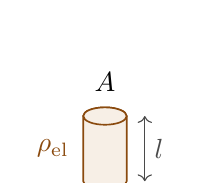
\begin{tikzpicture}[scale=0.92]
  \draw[koerper] (0,0) arc (180:360:0.3 and 0.12) -- (0.6,0.9) arc (0:180:0.3 and 0.12) -- cycle;
  \draw[koerper] (0.3,0.9) ellipse (0.3 and 0.12);
  \node[above] at (0.3,1.1) {$A$};
  \draw[<->,grau,line width=0.4pt] (0.85,0)--(0.85,0.9) node[midway,right]{$l$};
  \node[bern] at (-0.42,0.45) {$\rho_{\mathrm{el}}$};
\end{tikzpicture}
\fcap{\(R\) wächst mit \(l\), sinkt mit \(A\)}
\par}
\end{minipage}
\par\vspace{1.6mm}

\begin{minipage}[t]{0.54\linewidth}\vspace{0pt}
\ftitelD{Reihenschaltung}
\[ R_{\text{ges}} = R_1 + R_2 + \ldots \qquad I = I_1 = I_2 = \ldots \]
\[ U = U_1 + U_2 + \ldots \qquad \frac{U_1}{U_2} = \frac{R_1}{R_2} \]
\zwiD{Ohmsches Gesetz an jedem einzelnen Widerstand:}
\[ U_1 = R_1\cdot I_1 \qquad U_2 = R_2\cdot I_2 \qquad \mtxt{mit}\ \ I_1 = I_2 = I \]
\hinweis{Der Gesamtwiderstand ist \emph{grösser} als jeder Einzelwiderstand. Da überall derselbe Strom fliesst,
teilt sich die Spannung im Verhältnis der Widerstände auf -- \emph{Spannungsteiler}.}
\end{minipage}\hfill
\begin{minipage}[t]{0.44\linewidth}\vspace{0pt}
{\centering\tikzfont
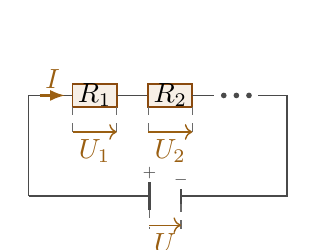
\begin{tikzpicture}[scale=0.80]
  \draw[grau,line width=0.6pt] (0,0)--(0,1.60)--(0.70,1.60);
  \draw[koerper] (0.70,1.42) rectangle (1.40,1.78); \node at (1.05,1.60) {$R_1$};
  \draw[grau,line width=0.6pt] (1.40,1.60)--(1.90,1.60);
  \draw[koerper] (1.90,1.42) rectangle (2.60,1.78); \node at (2.25,1.60) {$R_2$};
  \draw[grau,line width=0.6pt] (2.60,1.60)--(2.95,1.60);
  \foreach \x in {3.10,3.30,3.50}{\fill[grau] (\x,1.60) circle (0.045);}
  \draw[grau,line width=0.6pt] (3.65,1.60)--(4.10,1.60)--(4.10,0)--(2.42,0);
  \draw[grau,line width=0.6pt] (1.92,0)--(0,0);
  \draw[grau,line width=1pt] (1.92,-0.22)--(1.92,0.22);
  \draw[grau,line width=0.5pt] (2.42,-0.12)--(2.42,0.12);
  \node[grau,above,inner sep=1pt] at (1.92,0.22) {\tiny$+$};
  \node[grau,above,inner sep=1pt] at (2.42,0.12) {\tiny$-$};
  \draw[hilf] (1.92,-0.22)--(1.92,-0.52);
  \draw[hilf] (2.42,-0.12)--(2.42,-0.52);
  \draw[->,bernm,line width=0.5pt] (1.92,-0.46)--(2.42,-0.46);
  \node[bernm,below,inner sep=2pt] at (2.17,-0.50) {$U$};
  \draw[vecg,line width=0.8pt] (0.18,1.60)--(0.58,1.60);
  \node[bernm,above,inner sep=2pt] at (0.38,1.62) {$I$};
  \draw[hilf] (0.70,1.42)--(0.70,1.02); \draw[hilf] (1.40,1.42)--(1.40,1.02);
  \draw[->,bernm,line width=0.5pt] (0.70,1.02)--(1.40,1.02);
  \node[bernm,below,inner sep=2pt] at (1.05,1.00) {$U_1$};
  \draw[hilf] (1.90,1.42)--(1.90,1.02); \draw[hilf] (2.60,1.42)--(2.60,1.02);
  \draw[->,bernm,line width=0.5pt] (1.90,1.02)--(2.60,1.02);
  \node[bernm,below,inner sep=2pt] at (2.25,1.00) {$U_2$};
\end{tikzpicture}
\fcap{gleicher Strom, Spannung teilt sich auf -- weitere Widerstände folgen}
\par}
\end{minipage}
\par\vspace{1.6mm}

\begin{minipage}[t]{0.54\linewidth}\vspace{0pt}
\ftitelD{Parallelschaltung}
\[ \frac{1}{R_{\text{ges}}} = \frac{1}{R_1}+\frac{1}{R_2}+\ldots \qquad U = \mtxt{überall gleich} \]
\[ I = I_1 + I_2 + \ldots \qquad \frac{I_1}{I_2}=\frac{R_2}{R_1}
   \qquad R_{\text{ges}} = \frac{R_1 R_2}{R_1+R_2} \]
\zwiD{Ohmsches Gesetz in jedem einzelnen Zweig:}
\[ I_1 = \frac{U_1}{R_1} \qquad I_2 = \frac{U_2}{R_2} \qquad \mtxt{mit}\ \ U_1 = U_2 = U \]
\hinweis{Der Gesamtwiderstand ist \emph{kleiner} als der kleinste Einzelwiderstand. Da an allen Zweigen dieselbe
Spannung liegt, teilt sich der Strom umgekehrt zum Widerstand auf -- \emph{Stromteiler}.
Die Formel \(R_{\text{ges}} = R_1R_2/(R_1+R_2)\) gilt nur für \emph{zwei} Widerstände.}
\end{minipage}\hfill
\begin{minipage}[t]{0.44\linewidth}\vspace{0pt}
{\centering\tikzfont
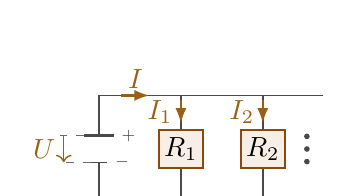
\begin{tikzpicture}[scale=0.80]
  \draw[grau,line width=0.6pt] (0,1.70)--(0,1.06);
  \draw[grau,line width=1pt]   (-0.24,1.06)--(0.24,1.06);
  \draw[grau,line width=0.5pt] (-0.13,0.64)--(0.13,0.64);
  \draw[grau,line width=0.6pt] (0,0.64)--(0,0);
  \node[grau,right,inner sep=2pt] at (0.26,1.06) {\tiny$+$};
  \node[grau,right,inner sep=2pt] at (0.15,0.64) {\tiny$-$};
  \draw[hilf] (-0.24,1.06)--(-0.62,1.06);
  \draw[hilf] (-0.13,0.64)--(-0.62,0.64);
  \draw[->,bernm,line width=0.5pt] (-0.56,1.06)--(-0.56,0.64);
  \node[bernm,left,inner sep=2pt] at (-0.60,0.85) {$U$};
  \draw[grau,line width=0.6pt] (0,1.70)--(3.55,1.70);
  \draw[grau,line width=0.6pt] (0,0)--(3.55,0);
  \draw[vecg,line width=0.8pt] (0.35,1.70)--(0.80,1.70);
  \node[bernm,above,inner sep=2pt] at (0.58,1.72) {$I$};
  \draw[grau,line width=0.6pt] (1.30,1.70)--(1.30,1.15);
  \draw[grau,line width=0.6pt] (1.30,0.55)--(1.30,0);
  \draw[koerper] (0.95,0.55) rectangle (1.65,1.15); \node at (1.30,0.85) {$R_1$};
  \draw[vecg,line width=0.8pt] (1.30,1.62)--(1.30,1.26);
  \node[bernm,left,inner sep=2pt] at (1.26,1.44) {$I_1$};
  \draw[grau,line width=0.6pt] (2.60,1.70)--(2.60,1.15);
  \draw[grau,line width=0.6pt] (2.60,0.55)--(2.60,0);
  \draw[koerper] (2.25,0.55) rectangle (2.95,1.15); \node at (2.60,0.85) {$R_2$};
  \draw[vecg,line width=0.8pt] (2.60,1.62)--(2.60,1.26);
  \node[bernm,left,inner sep=2pt] at (2.56,1.44) {$I_2$};
  \foreach \y in {0.65,0.85,1.05}{\fill[grau] (3.30,\y) circle (0.045);}
\end{tikzpicture}
\fcap{gleiche Spannung, Strom teilt sich auf -- weitere Zweige folgen}
\par}
\end{minipage}
\par\vspace{1.6mm}

\begin{minipage}[t]{0.54\linewidth}\vspace{0pt}
\needspace{4\baselineskip}\ftitelD{Elektrische Leistung und Energie}
\[ P = U\cdot I = R\cdot I^{\,2} = \frac{U^{\,2}}{R} \qquad\qquad E = P\cdot t = U\cdot I\cdot t \]
\gilt{\(P=U\,I\) gilt bei Gleichstrom allgemein. \(P=R\,I^2\) und \(P=U^2/R\) setzen einen ohmschen Widerstand voraus.
\(E=P\,t=U\,I\,t\) gilt bei konstanter Leistung bzw.\ konstanten Grössen.}
\hinweis{\(1\;\ME{kWh}=3.6\;\ME{MJ}\).}
\warn{Gefährlich ist die \emph{Stromstärke durch den Körper}. Schon wenige Milliampere sind spürbar und können
Muskelverkrampfungen auslösen; die Wirkung hängt von Stromstärke, Einwirkdauer, Stromweg durch den Körper und Frequenz ab.
Ein Fehlerstrom-Schutzschalter (FI/RCD) mit \(30\;\ME{mA}\) Auslösestrom ist eine \emph{zusätzliche} Schutzmassnahme --
keine Grenze für ungefährlichen Strom.}
% ======================================================================
\end{minipage}\hfill
\begin{minipage}[t]{0.44\linewidth}\vspace{0pt}
\begin{leg}
P & elektrische Leistung & W\\
E & elektrische Energie & J bzw.\ kWh
\end{leg}
\end{minipage}
\par\vspace{1.6mm}

\par\vspace{1.2mm}
\merk{\textbf{Elektrische Schutzmassnahmen.}
\textbf{Sicherung / Leitungsschutzschalter} -- schützt die \emph{Leitung} vor Überlast und Kurzschluss.\ \
\textbf{Schutzleiter (PE)} -- führt Fehlerstrom ab und ermöglicht zusammen mit der Schutzvorrichtung die automatische Abschaltung.\ \
\textbf{Schutzisolierung} -- doppelte Isolation, Gerät ohne Schutzleiter.\ \
\textbf{Fehlerstrom-Schutzschalter (FI/RCD)} -- erkennt bestimmte Fehlerströme und bietet \emph{zusätzlichen} Schutz vor elektrischem Schlag.\ \
\textbf{Schutzkleinspannung (SELV)} -- besonders niedrige Spannung zur deutlichen Verringerung des Risikos eines elektrischen Schlags.\ \
\textbf{Intakte Isolation} -- beschädigte Kabel und Stecker sofort ersetzen.}

\LG{A}{Anhang: Konstanten, Stoffwerte und Einheiten}

\begin{minipage}[t]{0.46\linewidth}\vspace{0pt}
\ftitel{Konstanten}
{\footnotesize\setlength{\tabcolsep}{4pt}\renewcommand{\arraystretch}{1.15}
\begin{tabular}[t]{@{}l l l@{}}
\rowcolor{bernl} Grösse & Symbol & Wert\\
Fallbeschleunigung (Erde) & \(g\) & \(9.81\;\ME{m/s^2}\)\\
Schallgeschw.\ (Luft, \(20\,^\circ\)C) & \(c_{\mathrm{S}}\) & \(343\;\ME{m/s}\)\\
Lichtgeschw.\ (Vakuum) & \(c\) & \(3.00\cdot10^{8}\;\ME{m/s}\)\\
Absoluter Nullpunkt & \(0\;\ME{K}\) & \(-273.15\,^\circ\ME{C}\)\\
Elementarladung & \(e\) & \(1.602\cdot10^{-19}\;\ME{C}\)\\
Planck-Konstante & \(h\) & \(6.626\cdot10^{-34}\;\ME{Js}\)\\
Coulomb-Konstante & \(k\) & \(8.99\cdot10^{9}\;\ME{Nm^2/C^2}\)\\
Kreiszahl & \(\pi\) & \(3.14159\ldots\)\\
Normluftdruck & \(p_0\) & \(1013\;\ME{hPa}\)\\
\end{tabular}}

\vspace{1.2mm}\ftitel{Stoffwerte (Richtwerte)}
{\footnotesize\setlength{\tabcolsep}{4pt}\renewcommand{\arraystretch}{1.15}
\begin{tabular}[t]{@{}l l l l@{}}
\rowcolor{bernl} Stoff & \(\rho\) [kg/m\(^3\)] & \(c\) [kJ/(kg\,K)] & \(\alpha\) [\(10^{-6}\)/K]\\
Wasser\(^{\ast}\) & 1000 & 4.19 & --\\
Eis & 917 & 2.1 & --\\
Luft (\(20\,^\circ\)C) & 1.20 & 1.0 & --\\
Aluminium & 2700 & 0.90 & 23\\
Eisen / Stahl & 7860 & 0.45 & 12\\
Kupfer & 8930 & 0.38 & 17\\
Beton & 2400 & 0.88 & 12\\
Holz (Fichte) & 500 & 2.1 & 5\\
\end{tabular}}
\hinweis{\(^{\ast}\)\,Wasser: \(\rho\) gilt bei \(4\,^\circ\)C (Dichtemaximum); \(c\) ist ein schulischer Richtwert
nahe \(20\,^\circ\)C.}
\hinweis{Wasser: \(L_{\text{f}} = 334\;\ME{kJ/kg}\) (bei \(0\,^\circ\)C), \(L_{\text{v}} = 2256\;\ME{kJ/kg}\) (bei \(100\,^\circ\)C, \(1013\;\ME{hPa}\)).}
\hinweis{\textbf{Zu den Werten:} Richtwerte bei \(20\,^\circ\)C und Normaldruck, sofern nicht anders angegeben.
Es sind gerundete \emph{schulische} Richtwerte; sie können je nach Quelle, Materialzusammensetzung und Bedingungen
abweichen -- besonders bei Legierungen, Beton und Holz. Für Berechnungen gelten die Angaben des Lehrmittels.}
\end{minipage}\hfill
\begin{minipage}[t]{0.50\linewidth}\vspace{0pt}
\ftitel{SI-Basiseinheiten}
{\footnotesize\setlength{\tabcolsep}{4pt}\renewcommand{\arraystretch}{1.15}
\begin{tabular}[t]{@{}l l l@{}}
\rowcolor{bernl} Grösse & Symbol & Einheit\\
Länge & \(l,s,h\) & Meter (m)\\
Masse & \(m\) & Kilogramm (kg)\\
Zeit & \(t\) & Sekunde (s)\\
Stromstärke & \(I\) & Ampere (A)\\
Temperatur & \(T\) & Kelvin (K)\\
Stoffmenge & \(n\) & Mol (mol)\\
Lichtstärke & \(I_v\) & Candela (cd)\\
\end{tabular}}

\vspace{1.2mm}\ftitel{Abgeleitete Einheiten}
{\footnotesize\setlength{\tabcolsep}{4pt}\renewcommand{\arraystretch}{1.15}
\begin{tabular}[t]{@{}l l l@{}}
\rowcolor{bernl} Grösse & Einheit & in Basiseinheiten\\
Kraft & Newton (N) & \(\ME{kg\,m/s^2}\)\\
Druck & Pascal (Pa) & \(\ME{N/m^2}=\ME{kg/(m\,s^2)}\)\\
Energie, Arbeit & Joule (J) & \(\ME{N\,m}=\ME{kg\,m^2/s^2}\)\\
Leistung & Watt (W) & \(\ME{J/s}\)\\
Frequenz & Hertz (Hz) & \(1/\ME{s}\)\\
Ladung & Coulomb (C) & \(\ME{A\,s}\)\\
Spannung & Volt (V) & \(\ME{J/C}=\ME{W/A}\)\\
Widerstand & Ohm (\(\Omega\)) & \(\ME{V/A}\)\\
Winkel & Radiant (rad) & \(\ME{m/m}\) (dimensionslos)\\
\end{tabular}}

\vspace{1.2mm}\ftitel{Praxiseinheiten mit Umrechnung}
{\footnotesize
\(1\;\ME{Pa}=1\;\ME{N/m^2}\)\quad
\(1\;\ME{kPa}=1000\;\ME{Pa}\)\quad
\(1\;\ME{hPa}=100\;\ME{Pa}\)\quad
\(1\;\ME{bar}=10^{5}\;\ME{Pa}\)\\
\(1\;\ME{Wh}=3600\;\ME{J}\)\quad
\(1\;\ME{kWh}=3.6\;\ME{MJ}\)\quad
\(1\;\ME{km/h}=\tfrac{1}{3.6}\;\ME{m/s}\)\\
\(1\;\ME{t}=1000\;\ME{kg}\)\quad
\(1\;\ME{l}=1\;\ME{dm^3}=10^{-3}\;\ME{m^3}\)\quad
\(\vartheta\,[^\circ\ME{C}] + 273.15 = T\,[\ME{K}]\)\par}
\end{minipage}

\par\vspace{2.5mm}
\par\vspace{1.5mm}\noindent{\color{bern}\bfseries\normalsize Symbolverzeichnis -- mehrfach verwendete Zeichen}%
\par\vspace{-1.4mm}{\color{bernm}\rule{\linewidth}{0.8pt}}\par\vspace{1.2mm}
{\footnotesize\setlength{\tabcolsep}{3pt}\renewcommand{\arraystretch}{1.05}
\begin{minipage}[t]{0.48\linewidth}\vspace{0pt}
\begin{tabular}[t]{@{}>{$}l<{$}@{\ \ }l l@{}}
\rowcolor{bernl} \mathrm{Zeichen} & Bedeutung & Einheit\\
a & Beschleunigung & m/s\(^2\)\\
\alpha & Längenausdehnungskoeffizient & \(\ME{K^{-1}}\)\\
c & Ausbreitungsgeschw.\ einer Welle & m/s\\
c & spezifische Wärmekapazität (Kap.\ 5) & J/(kg\,K)\\
c_{\mathrm{S}} & Schallgeschwindigkeit & m/s\\
s & Weg, Strecke & m\\
s & Verlängerung einer Feder (Hooke) & m\\
s_{\mathrm{b}} & Bogenlänge & m\\
\rho & Dichte & kg/m\(^3\)\\
\rho_{\mathrm{el}} & spezifischer Widerstand & \(\Omega\,\)m\\
\end{tabular}
\end{minipage}\hfill
\begin{minipage}[t]{0.48\linewidth}\vspace{0pt}
\begin{tabular}[t]{@{}>{$}l<{$}@{\ \ }l l@{}}
\rowcolor{bernl} \mathrm{Zeichen} & Bedeutung & Einheit\\
T & absolute Temperatur & K\\
T & Schwingungsdauer (Kap.\ 6) & s\\
\vartheta & Celsius-Temperatur & \(^\circ\)C\\
Q & Wärme (Kap.\ 5) & J\\
Q & elektrische Ladung (Kap.\ 6) & C\\
L & latente Wärme \(L_{\text{f}},L_{\text{v}}\) & J/kg\\
L & Länge der Saite (Kap.\ 6) & m\\
p & Druck & Pa\\
P & Leistung & W\\
\eta & Wirkungsgrad & --\\
\end{tabular}
\end{minipage}
\par}
\hinweis{Aufrechte Indizes stehen für \emph{Abkürzungen} (\(F_{\mathrm{G}}\) Gewichtskraft), kursive für \emph{Variablen und Richtungen}
(\(F_x\), \(\lambda_n\)). Welche Bedeutung gilt, zeigt das Kapitel.}

\vspace{2.5mm}
{\color{bernm}\rule{\linewidth}{0.8pt}}
\vspace{1mm}

\noindent
\begin{minipage}[t]{0.645\linewidth}\vspace{0pt}
{\footnotesize\color{grau}
\textbf{TALS Physik -- Formelsammlung.} Version 1.0 \ ·\ 1.~August 2026 \ ·\ Autor und Herausgeber: Raphael Arnold Kohler.
Formelsammlung zum Lehrmittel für die Berufsmaturität Technik, Architektur, Life Sciences (RLP-BM 2030).
Aufbau und Notation folgen den Themenseiten von
\href{https://go4exercises.github.io/TALS-Physik}{\nolinkurl{go4exercises.github.io/TALS-Physik}}.
Für Prüfungen gelten die von Schule, Kanton oder Prüfungsleitung festgelegten Hilfsmittel.\\[0.8mm]
Lizenz: \textbf{CC BY-NC 4.0} (Namensnennung -- nicht kommerziell), \url{https://creativecommons.org/licenses/by-nc/4.0/}\\[0.2mm]
Namensnennung bitte in der Form: \emph{Raphael Arnold Kohler: TALS Physik -- Formelsammlung, Version 1.0, CC BY-NC 4.0, go4exercises.github.io/TALS-Physik}\\[0.2mm]
Fehler und Rückmeldungen: \url{https://go4exercises.github.io/TALS-Physik/feedback.html}\\[0.4mm]
\textbf{Haftungsausschluss:} Alle Formeln, Werte und Darstellungen wurden sorgfältig erstellt und geprüft.
Dennoch wird keine Gewähr für Richtigkeit, Vollständigkeit und Aktualität übernommen.
Die Benutzung erfolgt auf eigene Verantwortung. Eine Haftung für Schäden aus der Verwendung dieser Unterlagen
wird im gesetzlich zulässigen Umfang ausgeschlossen. Zwingende gesetzliche Haftungsbestimmungen bleiben vorbehalten.\par}
\end{minipage}\hfill
\begin{minipage}[t]{0.335\linewidth}\vspace{0pt}
\centering\color{grau}\qrset{level=L,padding}
\begin{tabular}{@{}c@{\hspace{0.8mm}}c@{\hspace{0.8mm}}c@{}}
\qrcode[height=15mm]{https://go4exercises.github.io/TALS-Physik} &
\qrcode[height=15mm]{https://creativecommons.org/licenses/by-nc/4.0/} &
\qrcode[height=15mm]{https://go4exercises.github.io/TALS-Physik/feedback.html}\\[-0.6mm]
{\tiny Website} & {\tiny Lizenz} & {\tiny Feedback}
\end{tabular}
\end{minipage}\par

\end{document}
